\documentclass[11pt]{article}
\usepackage[review]{acl}
\usepackage{times}
\usepackage{latexsym}
\usepackage[T1]{fontenc}
\usepackage[utf8]{inputenc}
\usepackage{microtype}
\usepackage{inconsolata}
\usepackage{graphicx}
\usepackage{booktabs}
\usepackage{amsmath,amssymb,amsthm}
\usepackage{xcolor}
\usepackage{tikz}
\usetikzlibrary{arrows.meta,positioning}

\DeclareMathOperator*{\argmax}{arg\,max}

\newtheorem{proposition}{Proposition}
\newtheorem{lemma}{Lemma}
\newtheorem{corollary}{Corollary}
\newcommand{\rootnode}{\textsc{root}}
\newcommand{\method}{\textsc{TaxoBranch}}
\newcommand{\ef}{\textsc{eF1}}
\newcommand{\af}{\textsc{aF1}}
% Generated from validated contextual-baseline manifests; do not edit.
\newcommand{\BinaryEdge}{18.65$\pm$6.41}
\newcommand{\BinaryAncestor}{16.49$\pm$8.86}
\newcommand{\GraphEdge}{31.42$\pm$0.29}
\newcommand{\GraphAncestor}{17.33$\pm$0.27}
\newcommand{\TaxoTwentyEdge}{37.82$\pm$1.94}
\newcommand{\TaxoTwentyAncestor}{37.34$\pm$2.66}
\newcommand{\QwenEightEdge}{30.16}
\newcommand{\QwenEightAncestor}{21.73}
\newcommand{\QwenLargeEdge}{42.84}
\newcommand{\QwenLargeAncestor}{38.94}
\newcommand{\BoostOpenEdge}{42.12}
\newcommand{\BoostOpenAncestor}{40.54}
\newcommand{\TypedBinaryEdgeDelta}{19.42}
\newcommand{\TypedBinaryAncestorDelta}{24.37}
\newcommand{\TypedBinaryEdgeCILow}{13.60}
\newcommand{\TypedBinaryEdgeCIHigh}{25.58}
\newcommand{\TypedBinaryAncestorCILow}{14.79}
\newcommand{\TypedBinaryAncestorCIHigh}{31.50}
\newcommand{\OneParentCeiling}{99.32}
\newcommand{\CandidateOneParentCeiling}{84.02}
\newcommand{\ExactEdgeCILow}{0.004}
\newcommand{\ExactEdgeCIHigh}{0.048}
\newcommand{\ExactAncestorCILow}{-0.11}
\newcommand{\ExactAncestorCIHigh}{1.62}
\newcommand{\TensionChangeRho}{0.99}

% Generated from validated adaptive-allocation manifests; do not edit.
\newcommand{\AdaptiveFrozenBaseEdge}{37.74$\pm$1.17}
\newcommand{\AdaptiveFrozenEdge}{38.43$\pm$1.09}
\newcommand{\AdaptiveFrozenBaseAncestor}{34.88$\pm$1.96}
\newcommand{\AdaptiveFrozenAncestor}{36.38$\pm$2.13}
\newcommand{\AdaptiveFrozenEdgeGain}{0.69}
\newcommand{\AdaptiveFrozenAncestorGain}{1.50}
\newcommand{\AdaptiveFrozenPairFraction}{77.95}
\newcommand{\AdaptiveConfirmFixedEdge}{36.09$\pm$1.99}
\newcommand{\AdaptiveConfirmFixedAncestor}{30.93$\pm$4.92}
\newcommand{\AdaptiveConfirmCombinedEdge}{36.28$\pm$2.18}
\newcommand{\AdaptiveConfirmCombinedAncestor}{34.79$\pm$3.64}
\newcommand{\AdaptiveConfirmNeuralEdge}{36.32$\pm$2.21}
\newcommand{\AdaptiveConfirmNeuralAncestor}{33.38$\pm$4.40}
\newcommand{\AdaptiveConfirmSymbolicEdge}{36.58$\pm$1.83}
\newcommand{\AdaptiveConfirmSymbolicAncestor}{34.23$\pm$3.84}
\newcommand{\AdaptiveConfirmRandomEdge}{36.57$\pm$2.11}
\newcommand{\AdaptiveConfirmRandomAncestor}{33.25$\pm$4.41}
\newcommand{\AdaptiveConfirmUniformEdge}{36.66$\pm$2.27}
\newcommand{\AdaptiveConfirmUniformAncestor}{33.51$\pm$5.35}
\newcommand{\AdaptiveConfirmFullEdge}{36.55$\pm$2.24}
\newcommand{\AdaptiveConfirmFullAncestor}{36.16$\pm$3.15}
\newcommand{\AdaptiveConfirmEdgeGain}{0.19}
\newcommand{\AdaptiveConfirmEdgeCILow}{-0.10}
\newcommand{\AdaptiveConfirmEdgeCIHigh}{0.52}
\newcommand{\AdaptiveConfirmAncestorGain}{3.87}
\newcommand{\AdaptiveConfirmAncestorCILow}{1.55}
\newcommand{\AdaptiveConfirmAncestorCIHigh}{5.87}
\newcommand{\AdaptiveConfirmPairFraction}{74.92}
\newcommand{\AdaptiveConfirmPairSaving}{25.08}
\newcommand{\AdaptiveConfirmGPUFraction}{76.09}
\newcommand{\AdaptiveConfirmGPUSaving}{23.91}
\newcommand{\AdaptiveConfirmWallRatio}{100.58}
\newcommand{\AdaptiveConfirmAncestorRecovery}{73.89}
\newcommand{\AdaptiveConfirmCombinedGPUSeconds}{18.72}
\newcommand{\AdaptiveConfirmFullGPUSeconds}{24.60}
\newcommand{\AdaptiveConfirmCombinedPairs}{63,576}
\newcommand{\AdaptiveConfirmFullPairs}{84,860}
\newcommand{\AdaptiveConfirmValidOutputs}{210}
\newcommand{\AdaptiveConfirmBudgetCells}{30}
\newcommand{\AdaptiveConfirmActivationRate}{49.84}
\newcommand{\RootStandaloneDevF}{34.21$\pm$1.21}
\newcommand{\RootMarginDevF}{73.38$\pm$3.09}
\newcommand{\InputFull}{63.27$\pm$0.71}
\newcommand{\InputLabels}{37.37$\pm$5.04}
\newcommand{\InputDefinitions}{35.34$\pm$1.09}
\newcommand{\InputAnonymous}{19.09$\pm$7.72}
\newcommand{\AdaptiveConfirmScienceEdgeGain}{-0.10}
\newcommand{\AdaptiveConfirmScienceAncestorGain}{3.72}
\newcommand{\AdaptiveConfirmScienceEVEdgeGain}{0.43}
\newcommand{\AdaptiveConfirmScienceEVAncestorGain}{8.12}
\newcommand{\AdaptiveConfirmScienceWNEdgeGain}{-0.13}
\newcommand{\AdaptiveConfirmScienceWNAncestorGain}{5.37}
\newcommand{\AdaptiveConfirmEnvironmentEVEdgeGain}{0.25}
\newcommand{\AdaptiveConfirmEnvironmentEVAncestorGain}{1.61}
\newcommand{\AdaptiveConfirmFoodEdgeGain}{0.17}
\newcommand{\AdaptiveConfirmFoodAncestorGain}{2.01}
\newcommand{\AdaptiveConfirmFoodWNEdgeGain}{0.76}
\newcommand{\AdaptiveConfirmFoodWNAncestorGain}{8.35}

% Generated from validated value-of-computation manifests; do not edit.
\newcommand{\VoCConfirmSeeds}{10}
\newcommand{\VoCConfirmCells}{60}
\newcommand{\VoCConfirmValidOutputs}{420}
\newcommand{\VoCConfirmBudgetCells}{60}
\newcommand{\VoCAmendments}{2}
\newcommand{\VoCFiniteSeeds}{10}
\newcommand{\VoCFixedEdge}{36.77$\pm$1.91}
\newcommand{\VoCFixedAncestor}{32.08$\pm$2.41}
\newcommand{\VoCCombinedEdge}{38.00$\pm$2.34}
\newcommand{\VoCCombinedAncestor}{34.88$\pm$2.61}
\newcommand{\VoCNeuralEdge}{37.83$\pm$2.09}
\newcommand{\VoCNeuralAncestor}{34.59$\pm$1.94}
\newcommand{\VoCSymbolicEdge}{37.70$\pm$2.21}
\newcommand{\VoCSymbolicAncestor}{34.03$\pm$2.68}
\newcommand{\VoCRandomEdge}{37.02$\pm$2.15}
\newcommand{\VoCRandomAncestor}{32.67$\pm$2.62}
\newcommand{\VoCUniformEdge}{37.45$\pm$2.29}
\newcommand{\VoCUniformAncestor}{33.12$\pm$3.06}
\newcommand{\VoCFullEdge}{37.55$\pm$2.35}
\newcommand{\VoCFullAncestor}{34.53$\pm$2.21}
\newcommand{\VoCMinusFixedEdge}{1.23}
\newcommand{\VoCMinusFixedEdgeLow}{0.93}
\newcommand{\VoCMinusFixedEdgeHigh}{1.59}
\newcommand{\VoCMinusFixedEdgeWins}{10}
\newcommand{\VoCMinusFixedAncestor}{2.81}
\newcommand{\VoCMinusFixedAncestorLow}{2.12}
\newcommand{\VoCMinusFixedAncestorHigh}{3.62}
\newcommand{\VoCMinusFixedAncestorWins}{10}
\newcommand{\VoCMinusNeuralEdge}{0.17}
\newcommand{\VoCMinusNeuralEdgeLow}{-0.06}
\newcommand{\VoCMinusNeuralEdgeHigh}{0.41}
\newcommand{\VoCMinusNeuralEdgeWins}{5}
\newcommand{\VoCMinusNeuralAncestor}{0.29}
\newcommand{\VoCMinusNeuralAncestorLow}{-0.19}
\newcommand{\VoCMinusNeuralAncestorHigh}{0.76}
\newcommand{\VoCMinusNeuralAncestorWins}{7}
\newcommand{\VoCMinusSymbolicEdge}{0.30}
\newcommand{\VoCMinusSymbolicEdgeLow}{0.14}
\newcommand{\VoCMinusSymbolicEdgeHigh}{0.46}
\newcommand{\VoCMinusSymbolicEdgeWins}{9}
\newcommand{\VoCMinusSymbolicAncestor}{0.85}
\newcommand{\VoCMinusSymbolicAncestorLow}{0.21}
\newcommand{\VoCMinusSymbolicAncestorHigh}{1.57}
\newcommand{\VoCMinusSymbolicAncestorWins}{8}
\newcommand{\VoCMinusRandomEdge}{0.98}
\newcommand{\VoCMinusRandomEdgeLow}{0.69}
\newcommand{\VoCMinusRandomEdgeHigh}{1.26}
\newcommand{\VoCMinusRandomEdgeWins}{9}
\newcommand{\VoCMinusRandomAncestor}{2.21}
\newcommand{\VoCMinusRandomAncestorLow}{0.93}
\newcommand{\VoCMinusRandomAncestorHigh}{3.41}
\newcommand{\VoCMinusRandomAncestorWins}{8}
\newcommand{\VoCMinusUniformEdge}{0.55}
\newcommand{\VoCMinusUniformEdgeLow}{0.27}
\newcommand{\VoCMinusUniformEdgeHigh}{0.81}
\newcommand{\VoCMinusUniformEdgeWins}{8}
\newcommand{\VoCMinusUniformAncestor}{1.77}
\newcommand{\VoCMinusUniformAncestorLow}{1.23}
\newcommand{\VoCMinusUniformAncestorHigh}{2.35}
\newcommand{\VoCMinusUniformAncestorWins}{10}
\newcommand{\VoCMinusFullEdge}{0.45}
\newcommand{\VoCMinusFullEdgeLow}{0.28}
\newcommand{\VoCMinusFullEdgeHigh}{0.62}
\newcommand{\VoCMinusFullEdgeWins}{9}
\newcommand{\VoCMinusFullAncestor}{0.36}
\newcommand{\VoCMinusFullAncestorLow}{-0.02}
\newcommand{\VoCMinusFullAncestorHigh}{0.83}
\newcommand{\VoCMinusFullAncestorWins}{5}
\newcommand{\VoCPairFraction}{75.00}
\newcommand{\VoCPairSaving}{25.00}
\newcommand{\VoCGPUFraction}{76.49}
\newcommand{\VoCGPUSaving}{23.51}
\newcommand{\VoCWallFraction}{76.29}
\newcommand{\VoCWallSaving}{23.71}
\newcommand{\VoCCombinedPairs}{63,645}
\newcommand{\VoCFullPairs}{84,860}
\newcommand{\VoCCombinedGPUSeconds}{11.74}
\newcommand{\VoCFullGPUSeconds}{15.35}
\newcommand{\VoCCombinedWallSeconds}{20.84}
\newcommand{\VoCFullWallSeconds}{28.40}
\newcommand{\VoCSymbolicMinusFixedEdge}{0.93}
\newcommand{\VoCSymbolicMinusFixedEdgeLow}{0.61}
\newcommand{\VoCSymbolicMinusFixedEdgeHigh}{1.30}
\newcommand{\VoCSymbolicMinusFixedEdgeWins}{10}
\newcommand{\VoCSymbolicMinusFixedAncestor}{1.96}
\newcommand{\VoCSymbolicMinusFixedAncestorLow}{0.78}
\newcommand{\VoCSymbolicMinusFixedAncestorHigh}{3.15}
\newcommand{\VoCSymbolicMinusFixedAncestorWins}{8}
\newcommand{\VoCSymbolicMinusRandomEdge}{0.68}
\newcommand{\VoCSymbolicMinusRandomEdgeLow}{0.37}
\newcommand{\VoCSymbolicMinusRandomEdgeHigh}{0.98}
\newcommand{\VoCSymbolicMinusRandomEdgeWins}{9}
\newcommand{\VoCSymbolicMinusRandomAncestor}{1.36}
\newcommand{\VoCSymbolicMinusRandomAncestorLow}{-0.18}
\newcommand{\VoCSymbolicMinusRandomAncestorHigh}{2.75}
\newcommand{\VoCSymbolicMinusRandomAncestorWins}{8}
\newcommand{\VoCSymbolicMinusUniformEdge}{0.25}
\newcommand{\VoCSymbolicMinusUniformEdgeLow}{-0.03}
\newcommand{\VoCSymbolicMinusUniformEdgeHigh}{0.51}
\newcommand{\VoCSymbolicMinusUniformEdgeWins}{8}
\newcommand{\VoCSymbolicMinusUniformAncestor}{0.92}
\newcommand{\VoCSymbolicMinusUniformAncestorLow}{0.05}
\newcommand{\VoCSymbolicMinusUniformAncestorHigh}{1.84}
\newcommand{\VoCSymbolicMinusUniformAncestorWins}{8}
\newcommand{\VoCSymbolicMinusFullEdge}{0.15}
\newcommand{\VoCSymbolicMinusFullEdgeLow}{0.03}
\newcommand{\VoCSymbolicMinusFullEdgeHigh}{0.29}
\newcommand{\VoCSymbolicMinusFullEdgeWins}{7}
\newcommand{\VoCSymbolicMinusFullAncestor}{-0.49}
\newcommand{\VoCSymbolicMinusFullAncestorLow}{-1.44}
\newcommand{\VoCSymbolicMinusFullAncestorHigh}{0.37}
\newcommand{\VoCSymbolicMinusFullAncestorWins}{5}
\newcommand{\VoCWallSavingLow}{20.94}
\newcommand{\VoCWallSavingHigh}{27.39}
\newcommand{\VoCWallSavingWins}{10}
\newcommand{\VoCGPUSavingLow}{23.12}
\newcommand{\VoCGPUSavingHigh}{23.94}
\newcommand{\VoCGPUSavingWins}{10}
\newcommand{\VoCEdgeRecovery}{158.08}
\newcommand{\VoCAncestorRecovery}{114.50}
\newcommand{\VoCScienceEdgeGain}{0.51}
\newcommand{\VoCScienceEdgeLow}{0.15}
\newcommand{\VoCScienceEdgeHigh}{0.86}
\newcommand{\VoCScienceAncestorGain}{2.97}
\newcommand{\VoCScienceAncestorLow}{0.37}
\newcommand{\VoCScienceAncestorHigh}{5.26}
\newcommand{\VoCScienceEVEdgeGain}{2.74}
\newcommand{\VoCScienceEVEdgeLow}{1.74}
\newcommand{\VoCScienceEVEdgeHigh}{3.93}
\newcommand{\VoCScienceEVAncestorGain}{6.68}
\newcommand{\VoCScienceEVAncestorLow}{4.57}
\newcommand{\VoCScienceEVAncestorHigh}{8.48}
\newcommand{\VoCEnvironmentEVEdgeGain}{0.95}
\newcommand{\VoCEnvironmentEVEdgeLow}{0.32}
\newcommand{\VoCEnvironmentEVEdgeHigh}{1.58}
\newcommand{\VoCEnvironmentEVAncestorGain}{0.68}
\newcommand{\VoCEnvironmentEVAncestorLow}{-0.86}
\newcommand{\VoCEnvironmentEVAncestorHigh}{2.66}
\newcommand{\VoCFoodEdgeGain}{0.73}
\newcommand{\VoCFoodEdgeLow}{0.58}
\newcommand{\VoCFoodEdgeHigh}{0.89}
\newcommand{\VoCFoodAncestorGain}{0.89}
\newcommand{\VoCFoodAncestorLow}{-0.84}
\newcommand{\VoCFoodAncestorHigh}{2.41}
\newcommand{\VoCScienceWNEdgeGain}{1.52}
\newcommand{\VoCScienceWNEdgeLow}{0.85}
\newcommand{\VoCScienceWNEdgeHigh}{2.10}
\newcommand{\VoCScienceWNAncestorGain}{9.48}
\newcommand{\VoCScienceWNAncestorLow}{8.18}
\newcommand{\VoCScienceWNAncestorHigh}{10.91}
\newcommand{\VoCFoodWNEdgeGain}{1.27}
\newcommand{\VoCFoodWNEdgeLow}{1.12}
\newcommand{\VoCFoodWNEdgeHigh}{1.43}
\newcommand{\VoCFoodWNAncestorGain}{13.37}
\newcommand{\VoCFoodWNAncestorLow}{10.71}
\newcommand{\VoCFoodWNAncestorHigh}{15.30}
\newcommand{\VoCModelLoadSeconds}{16.70}
\newcommand{\VoCDevCalibrationGPUSeconds}{137.87}

% Generated from validated allocation-precursor manifests; do not edit.
\newcommand{\PrimaryFixedEdge}{35.54}
\newcommand{\PrimaryFixedAncestor}{29.28}
\newcommand{\PrimaryRandomEdge}{35.52}
\newcommand{\PrimaryRandomAncestor}{32.24}
\newcommand{\PrimaryUniformEdge}{35.91}
\newcommand{\PrimaryUniformAncestor}{30.65}
\newcommand{\PrimarySymbolicEdge}{36.13}
\newcommand{\PrimarySymbolicAncestor}{32.28}
\newcommand{\PrimaryNeuralEdge}{35.99}
\newcommand{\PrimaryNeuralAncestor}{33.51}
\newcommand{\PrimaryCombinedEdge}{36.17}
\newcommand{\PrimaryCombinedAncestor}{33.47}
\newcommand{\PrimaryFullEdge}{35.97}
\newcommand{\PrimaryFullAncestor}{33.69}
\newcommand{\PrimaryMinusFixedEdge}{0.63}
\newcommand{\PrimaryMinusFixedEdgeLow}{0.15}
\newcommand{\PrimaryMinusFixedEdgeHigh}{1.03}
\newcommand{\PrimaryMinusFixedAncestor}{4.19}
\newcommand{\PrimaryMinusFixedAncestorLow}{2.72}
\newcommand{\PrimaryMinusFixedAncestorHigh}{5.81}
\newcommand{\PrimaryMinusNeuralEdge}{0.19}
\newcommand{\PrimaryMinusNeuralEdgeLow}{0.02}
\newcommand{\PrimaryMinusNeuralEdgeHigh}{0.37}
\newcommand{\PrimaryMinusNeuralAncestor}{-0.04}
\newcommand{\PrimaryMinusNeuralAncestorLow}{-1.04}
\newcommand{\PrimaryMinusNeuralAncestorHigh}{0.60}
\newcommand{\PrimaryMinusSymbolicEdge}{0.04}
\newcommand{\PrimaryMinusSymbolicEdgeLow}{-0.12}
\newcommand{\PrimaryMinusSymbolicEdgeHigh}{0.21}
\newcommand{\PrimaryMinusSymbolicAncestor}{1.19}
\newcommand{\PrimaryMinusSymbolicAncestorLow}{0.15}
\newcommand{\PrimaryMinusSymbolicAncestorHigh}{2.26}
\newcommand{\PrimaryMinusFullEdge}{0.20}
\newcommand{\PrimaryMinusFullEdgeLow}{-0.06}
\newcommand{\PrimaryMinusFullEdgeHigh}{0.49}
\newcommand{\PrimaryMinusFullAncestor}{-0.22}
\newcommand{\PrimaryMinusFullAncestorLow}{-1.27}
\newcommand{\PrimaryMinusFullAncestorHigh}{0.42}
\newcommand{\PrimaryGPUSaving}{24.31}
\newcommand{\PrimaryWallSaving}{21.06}
\newcommand{\PrimaryPairSaving}{25}
\newcommand{\PrimaryValidOutputs}{420}
\newcommand{\PrimaryBudgetCells}{60}

% Generated from validated hierarchy-allocation manifests; do not edit.
\newcommand{\HierarchyAuditSeeds}{10}
\newcommand{\HierarchyAuditValidOutputs}{1,740}
\newcommand{\HierarchySymbolicMinusRandomEdge}{0.57}
\newcommand{\HierarchySymbolicMinusRandomEdgeLow}{0.40}
\newcommand{\HierarchySymbolicMinusRandomEdgeHigh}{0.74}
\newcommand{\HierarchySymbolicMinusRandomEdgeWins}{10}
\newcommand{\HierarchySymbolicMinusUniformEdge}{0.22}
\newcommand{\HierarchySymbolicMinusUniformEdgeLow}{0.09}
\newcommand{\HierarchySymbolicMinusUniformEdgeHigh}{0.34}
\newcommand{\HierarchySymbolicMinusUniformAncestor}{1.76}
\newcommand{\HierarchySymbolicMinusUniformAncestorLow}{0.14}
\newcommand{\HierarchySymbolicMinusUniformAncestorHigh}{3.36}
\newcommand{\HierarchyNetRepairEnrichment}{1.51}
\newcommand{\HierarchyNetRepairEnrichmentLow}{0.52}
\newcommand{\HierarchyNetRepairEnrichmentHigh}{2.31}
\newcommand{\HierarchyNetRepairEnrichmentWins}{9}

% Generated from validated retrieval-stress manifests; do not edit.
\newcommand{\ProjectionStressSeeds}{10}
\newcommand{\ProjectionStressBaseLocalValid}{27.50}
\newcommand{\ProjectionStressBaseExactValid}{100.00}
\newcommand{\ProjectionStressBaseEditRate}{0.99}
\newcommand{\ProjectionStressBaseCyclicNodes}{14.50}
\newcommand{\ProjectionStressBaseTension}{0.0041}
\newcommand{\ProjectionStressBaseEdge}{36.07}
\newcommand{\ProjectionStressBaseAncestor}{34.88}
\newcommand{\ProjectionStressHighLocalValid}{27.50}
\newcommand{\ProjectionStressHighExactValid}{100.00}
\newcommand{\ProjectionStressHighEditRate}{0.98}
\newcommand{\ProjectionStressHighTension}{0.0223}
\newcommand{\ProjectionStressHighEdge}{36.09}
\newcommand{\ProjectionStressHighAncestor}{35.14}
\newcommand{\ProjectionStressHighMinusBaseEdge}{+0.02}
\newcommand{\ProjectionStressHighMinusBaseAncestor}{+0.26}
\newcommand{\ProjectionStressTensionEditSpearman}{0.907}
\newcommand{\RetrievalStressKFiveRecall}{48.41}
\newcommand{\RetrievalStressKFiveCeiling}{62.67}
\newcommand{\RetrievalStressKFiveLocalValid}{5.00}
\newcommand{\RetrievalStressKFiveExactValid}{100.00}
\newcommand{\RetrievalStressKFiveEdge}{34.42}
\newcommand{\RetrievalStressKFiveAncestor}{31.41}
\newcommand{\RetrievalStressKTenRecall}{59.53}
\newcommand{\RetrievalStressKTenCeiling}{71.51}
\newcommand{\RetrievalStressKTenLocalValid}{7.50}
\newcommand{\RetrievalStressKTenExactValid}{100.00}
\newcommand{\RetrievalStressKTenEdge}{35.72}
\newcommand{\RetrievalStressKTenAncestor}{32.43}
\newcommand{\RetrievalStressKTwentyRecall}{69.05}
\newcommand{\RetrievalStressKTwentyCeiling}{78.29}
\newcommand{\RetrievalStressKTwentyLocalValid}{27.50}
\newcommand{\RetrievalStressKTwentyExactValid}{100.00}
\newcommand{\RetrievalStressKTwentyEdge}{36.07}
\newcommand{\RetrievalStressKTwentyAncestor}{34.88}
\newcommand{\ProjectionAuditCells}{40}
\newcommand{\ProjectionAuditBaseInvalid}{29}
\newcommand{\ProjectionAuditBaseEditsMean}{7.08}
\newcommand{\ProjectionAuditBaseEditsMedian}{2.00}
\newcommand{\ProjectionAuditBaseEditRateMean}{0.99}
\newcommand{\ProjectionAuditBaseEditRatePninety}{2.31}
\newcommand{\ProjectionAuditBaseCyclicMean}{14.50}
\newcommand{\ProjectionAuditBaseCyclicPninety}{33.90}
\newcommand{\ProjectionAuditBaseTensionMean}{2.70}
\newcommand{\ProjectionAuditBaseTensionMedian}{1.26}
\newcommand{\ProjectionAuditBaseTensionPninety}{6.26}
\newcommand{\ProjectionAuditHighInvalid}{29}
\newcommand{\ProjectionAuditHighEditsMean}{7.00}
\newcommand{\ProjectionAuditHighEditsMedian}{2.00}
\newcommand{\ProjectionAuditHighEditRateMean}{0.98}
\newcommand{\ProjectionAuditHighEditRatePninety}{2.31}
\newcommand{\ProjectionAuditHighCyclicMean}{14.50}
\newcommand{\ProjectionAuditHighCyclicPninety}{33.90}
\newcommand{\ProjectionAuditHighTensionMean}{15.64}
\newcommand{\ProjectionAuditHighTensionMedian}{5.53}
\newcommand{\ProjectionAuditHighTensionPninety}{36.29}

% Generated; do not edit.
\newcommand{\PressureRuns}{1280}
\newcommand{\PressureCells}{64}
\newcommand{\PressureExactValid}{100.0}
\newcommand{\PressureGreedyRegret}{2.65}
\newcommand{\PressureMinimalRegret}{2.55}
\newcommand{\PressureExactRegret}{0.00}
\newcommand{\PressureOverlapGreedyRegret}{5.23}
\newcommand{\PressureOverlapMinimalRegret}{5.10}
\newcommand{\PressureOverlapExactRegret}{0.00}
\newcommand{\PressureGreedyEdits}{4.53}
\newcommand{\PressureMinimalEdits}{4.53}
\newcommand{\PressureExactEdits}{5.59}
\newcommand{\PressureGreedyMillis}{19.1}
\newcommand{\PressureMinimalMillis}{22.2}
\newcommand{\PressureExactMillis}{21.2}

% Post-primary frozen-score multi-parent DAG extension, seeds 67--76.
\newcommand{\DagForestEdge}{36.07}
\newcommand{\DagForestAncestor}{34.88}
\newcommand{\DagAccuracyEdge}{36.07}
\newcommand{\DagAccuracyAncestor}{34.88}
\newcommand{\DagMultiEdge}{36.10}
\newcommand{\DagMultiAncestor}{34.87}
\newcommand{\DagMultiEdgeDelta}{+0.03}
\newcommand{\DagMultiEdgeDeltaLow}{-0.06}
\newcommand{\DagMultiEdgeDeltaHigh}{+0.14}
\newcommand{\DagMultiAncestorDelta}{-0.01}
\newcommand{\DagMultiAncestorDeltaLow}{-0.06}
\newcommand{\DagMultiAncestorDeltaHigh}{+0.04}
\newcommand{\DagMultiPrecision}{0.40}
\newcommand{\DagMultiRecall}{0.43}
\newcommand{\DagMultiFone}{0.42}
\newcommand{\DagMultiPredicted}{30.6}
\newcommand{\DagMultiGold}{46.0}
\newcommand{\DagMultiTruePositive}{0.2}
\newcommand{\DagCapFraction}{2.07}
\newcommand{\DagValidOutputs}{80}
\newcommand{\DagAccuracyThresholdZeroSeeds}{9}
\newcommand{\DagMultiThresholdMin}{-0.250}
\newcommand{\DagMultiThresholdMax}{-0.050}

% Frozen retrieval ceilings for Macro4 multi-parent children.
\newcommand{\MpOracleGoldChildren}{46}
\newcommand{\MpOracleCompleteTwenty}{11}
\newcommand{\MpOracleCompleteTwentyRate}{23.9}
\newcommand{\MpOracleCompleteFifty}{17}
\newcommand{\MpOracleCompleteFiftyRate}{37.0}
\newcommand{\MpOracleFoodTwenty}{2}
\newcommand{\MpOracleFoodGold}{32}

% Sealed post-outcome symmetric semantic pair-reranker, seeds 67--76.
\newcommand{\PairMacroFourBaselineEdge}{36.15}
\newcommand{\PairMacroFourSemanticEdge}{37.00}
\newcommand{\PairMacroFourEdgeDelta}{+0.86}
\newcommand{\PairMacroFourEdgeLow}{+0.44}
\newcommand{\PairMacroFourEdgeHigh}{+1.28}
\newcommand{\PairMacroFourEdgeP}{.008}
\newcommand{\PairMacroFourEdgeWins}{9}
\newcommand{\PairMacroFourBaselineAncestor}{44.85}
\newcommand{\PairMacroFourSemanticAncestor}{45.72}
\newcommand{\PairMacroFourAncestorDelta}{+0.87}
\newcommand{\PairMacroFourAncestorLow}{+0.19}
\newcommand{\PairMacroFourAncestorHigh}{+1.67}
\newcommand{\PairMacroFourAncestorP}{.049}
\newcommand{\PairMacroFourAncestorWins}{8}
\newcommand{\PairMacroFourScalarPairRecallOne}{0.00}
\newcommand{\PairMacroFourSemanticPairRecallOne}{7.86}
\newcommand{\PairMacroFourPairRecallDelta}{+7.86}
\newcommand{\PairMacroFourPairRecallLow}{+3.57}
\newcommand{\PairMacroFourPairRecallHigh}{+12.14}
\newcommand{\PairMacroFourPairRecallP}{.016}
\newcommand{\PairMacroFourPairRecallWins}{7}
\newcommand{\PairMacroSixBaselineEdge}{35.07}
\newcommand{\PairMacroSixSemanticEdge}{36.05}
\newcommand{\PairMacroSixEdgeDelta}{+0.98}
\newcommand{\PairMacroSixEdgeLow}{+0.56}
\newcommand{\PairMacroSixEdgeHigh}{+1.38}
\newcommand{\PairMacroSixEdgeP}{.006}
\newcommand{\PairMacroSixEdgeWins}{9}
\newcommand{\PairMacroSixBaselineAncestor}{42.17}
\newcommand{\PairMacroSixSemanticAncestor}{42.90}
\newcommand{\PairMacroSixAncestorDelta}{+0.73}
\newcommand{\PairMacroSixAncestorLow}{+0.25}
\newcommand{\PairMacroSixAncestorHigh}{+1.34}
\newcommand{\PairMacroSixAncestorP}{.006}
\newcommand{\PairMacroSixAncestorWins}{9}
\newcommand{\PairMacroSixScalarPairRecallOne}{0.00}
\newcommand{\PairMacroSixSemanticPairRecallOne}{7.65}
\newcommand{\PairMacroSixPairRecallDelta}{+7.65}
\newcommand{\PairMacroSixPairRecallLow}{+4.41}
\newcommand{\PairMacroSixPairRecallHigh}{+10.88}
\newcommand{\PairMacroSixPairRecallP}{.008}
\newcommand{\PairMacroSixPairRecallWins}{8}
\newcommand{\PairTransformerForwards}{0}
\newcommand{\PairSeeds}{10}

% Generated from validated parent-set manifests; do not edit.
\newcommand{\JointSetSeeds}{10}
\newcommand{\JointAdaptivePairs}{9.3}
\newcommand{\JointQThreeSavingAdaptive}{67.7}
\newcommand{\JointQThreeSavingQFive}{70.0}
\newcommand{\JointQThreeSavingQTen}{93.3}
\newcommand{\JointQThreePairs}{3}
\newcommand{\JointQFivePairs}{10}
\newcommand{\JointQTenPairs}{45}
\newcommand{\JointHybridQThreeExact}{0.375}
\newcommand{\JointHybridQThreeEdge}{39.25}
\newcommand{\JointHybridQThreeAncestor}{46.90}
\newcommand{\JointHybridQFiveExact}{0.361}
\newcommand{\JointHybridQFiveEdge}{39.16}
\newcommand{\JointHybridQFiveAncestor}{46.68}
\newcommand{\JointHybridQTenExact}{0.359}
\newcommand{\JointHybridQTenEdge}{39.22}
\newcommand{\JointHybridQTenAncestor}{46.74}
\newcommand{\JointHybridAdaptiveExact}{0.368}
\newcommand{\JointHybridAdaptiveEdge}{39.19}
\newcommand{\JointHybridAdaptiveAncestor}{46.88}
\newcommand{\JointLearnedQThreeExact}{0.334}
\newcommand{\JointLearnedQThreeEdge}{39.43}
\newcommand{\JointLearnedQThreeAncestor}{42.39}
\newcommand{\JointLearnedQFiveExact}{0.311}
\newcommand{\JointLearnedQFiveEdge}{39.35}
\newcommand{\JointLearnedQFiveAncestor}{42.23}
\newcommand{\JointLearnedQTenExact}{0.305}
\newcommand{\JointLearnedQTenEdge}{39.24}
\newcommand{\JointLearnedQTenAncestor}{42.20}
\newcommand{\JointLearnedAdaptiveExact}{0.314}
\newcommand{\JointLearnedAdaptiveEdge}{39.28}
\newcommand{\JointLearnedAdaptiveAncestor}{42.20}
\newcommand{\JointPrimaryReferenceExact}{0.361}
\newcommand{\JointPrimaryCandidateExact}{0.314}
\newcommand{\JointPrimaryExactDelta}{-0.05}
\newcommand{\JointPrimaryExactP}{1.000}

% Generated from validated allocation and transfer manifests; do not edit.
\newcommand{\NISeeds}{30}
\newcommand{\NICombinedEdge}{38.59}
\newcommand{\NICombinedAncestor}{34.70}
\newcommand{\NIFullEdge}{38.26}
\newcommand{\NIFullAncestor}{35.01}
\newcommand{\NIEdgeDiff}{+0.32}
\newcommand{\NIEdgeLower}{+0.20}
\newcommand{\NIEdgeMargin}{0.50}
\newcommand{\NIAncestorDiff}{-0.31}
\newcommand{\NIAncestorLower}{-0.66}
\newcommand{\NIAncestorMargin}{1.00}
\newcommand{\NIPairSaving}{25.00}
\newcommand{\NIGPUSaving}{23.69}
\newcommand{\NIWallSaving}{20.79}
\newcommand{\NIMinusNeuralEdge}{+0.15}
\newcommand{\NIMinusNeuralEdgeLow}{+0.05}
\newcommand{\NIMinusNeuralEdgeHigh}{+0.25}
\newcommand{\NIMinusNeuralAncestor}{-0.27}
\newcommand{\NIMinusNeuralAncestorLow}{-0.70}
\newcommand{\NIMinusNeuralAncestorHigh}{+0.09}
\newcommand{\MatchedTypedEdge}{38.52$\pm$2.07}
\newcommand{\MatchedTypedAncestor}{33.88$\pm$3.11}
\newcommand{\MatchedBinaryEdge}{26.71$\pm$3.04}
\newcommand{\MatchedBinaryAncestor}{28.02$\pm$5.15}
\newcommand{\MatchedPairwiseEdge}{29.96$\pm$3.59}
\newcommand{\MatchedPairwiseAncestor}{24.13$\pm$3.89}
\newcommand{\TypedMinusBinaryEdge}{+11.81}
\newcommand{\TypedMinusBinaryEdgeLow}{+9.88}
\newcommand{\TypedMinusBinaryEdgeHigh}{+13.57}
\newcommand{\TypedMinusBinaryAncestor}{+5.86}
\newcommand{\TypedMinusBinaryAncestorLow}{+2.04}
\newcommand{\TypedMinusBinaryAncestorHigh}{+9.37}
\newcommand{\TypedMinusPairwiseEdge}{+8.56}
\newcommand{\TypedMinusPairwiseEdgeLow}{+6.19}
\newcommand{\TypedMinusPairwiseEdgeHigh}{+11.11}
\newcommand{\TypedMinusPairwiseAncestor}{+9.75}
\newcommand{\TypedMinusPairwiseAncestorLow}{+7.09}
\newcommand{\TypedMinusPairwiseAncestorHigh}{+12.16}
\newcommand{\SchemaTypedEdge}{28.57$\pm$5.72}
\newcommand{\SchemaLexicalEdge}{3.96}
\newcommand{\SchemaTypedAncestor}{15.57$\pm$6.07}
\newcommand{\SchemaLexicalAncestor}{0.47}
\newcommand{\SchemaValid}{100.0}
\newcommand{\MAGCSMRR}{0.132$\pm$0.014}
\newcommand{\MAGCSRetrievalMRR}{0.151}
\newcommand{\MAGCSAcc}{0.093$\pm$0.014}
\newcommand{\MAGCSRetrievalAcc}{0.099}
\newcommand{\MAGCSCeiling}{0.563}
\newcommand{\MAGPSYMRR}{0.168$\pm$0.022}
\newcommand{\MAGPSYRetrievalMRR}{0.145}
\newcommand{\MAGPSYAcc}{0.121$\pm$0.020}
\newcommand{\MAGPSYRetrievalAcc}{0.080}
\newcommand{\MAGPSYCeiling}{0.543}
\newcommand{\CertSeeds}{10}
\newcommand{\CertPairFraction}{75}
\newcommand{\CertValid}{100.0}
\newcommand{\CertExtraTransformerPairs}{0}
\newcommand{\CertFixedEdge}{37.99$\pm$1.55}
\newcommand{\CertFixedAncestor}{31.37$\pm$3.90}
\newcommand{\CertOnlyEdge}{38.60$\pm$1.91}
\newcommand{\CertOnlyAncestor}{33.73$\pm$2.73}
\newcommand{\CertNeuralEdge}{38.54$\pm$2.08}
\newcommand{\CertNeuralAncestor}{33.73$\pm$3.21}
\newcommand{\CertLocalEdge}{38.81$\pm$2.22}
\newcommand{\CertLocalAncestor}{33.81$\pm$2.90}
\newcommand{\CertPlusEdge}{38.60$\pm$2.07}
\newcommand{\CertPlusAncestor}{33.45$\pm$3.00}
\newcommand{\CertRandomEdge}{38.26$\pm$1.92}
\newcommand{\CertRandomAncestor}{32.47$\pm$3.67}
\newcommand{\CertUniformEdge}{38.46$\pm$1.78}
\newcommand{\CertUniformAncestor}{32.38$\pm$3.02}
\newcommand{\CertFullEdge}{38.52$\pm$2.07}
\newcommand{\CertFullAncestor}{33.88$\pm$3.11}
\newcommand{\CertPlusMinusNeuralEdge}{+0.07}
\newcommand{\CertPlusMinusNeuralEdgeLow}{-0.11}
\newcommand{\CertPlusMinusNeuralEdgeHigh}{+0.26}
\newcommand{\CertPlusMinusNeuralAncestor}{-0.27}
\newcommand{\CertPlusMinusNeuralAncestorLow}{-0.87}
\newcommand{\CertPlusMinusNeuralAncestorHigh}{+0.10}
\newcommand{\CertPlusMinusLocalEdge}{-0.21}
\newcommand{\CertPlusMinusLocalEdgeLow}{-0.43}
\newcommand{\CertPlusMinusLocalEdgeHigh}{+0.04}
\newcommand{\CertPlusMinusLocalAncestor}{-0.35}
\newcommand{\CertPlusMinusLocalAncestorLow}{-1.09}
\newcommand{\CertPlusMinusLocalAncestorHigh}{+0.24}
\newcommand{\CertOnlyMinusFixedEdge}{+0.61}
\newcommand{\CertOnlyMinusFixedEdgeLow}{+0.28}
\newcommand{\CertOnlyMinusFixedEdgeHigh}{+0.92}
\newcommand{\CertOnlyMinusFixedAncestor}{+2.36}
\newcommand{\CertOnlyMinusFixedAncestorLow}{+0.95}
\newcommand{\CertOnlyMinusFixedAncestorHigh}{+3.95}
\newcommand{\CertOnlyMinusRandomEdge}{+0.35}
\newcommand{\CertOnlyMinusRandomEdgeLow}{+0.11}
\newcommand{\CertOnlyMinusRandomEdgeHigh}{+0.60}
\newcommand{\CertOnlyMinusRandomAncestor}{+1.27}
\newcommand{\CertOnlyMinusRandomAncestorLow}{-0.04}
\newcommand{\CertOnlyMinusRandomAncestorHigh}{+2.58}
\newcommand{\CertOnlyMinusUniformEdge}{+0.14}
\newcommand{\CertOnlyMinusUniformEdgeLow}{-0.12}
\newcommand{\CertOnlyMinusUniformEdgeHigh}{+0.39}
\newcommand{\CertOnlyMinusUniformAncestor}{+1.35}
\newcommand{\CertOnlyMinusUniformAncestorLow}{+0.27}
\newcommand{\CertOnlyMinusUniformAncestorHigh}{+2.41}

% Generated from validated Schema.org transfer manifests; do not edit.
\newcommand{\SchemaTransferSchemaSeeds}{10}
\newcommand{\SchemaTransferSchemaTypedEdge}{31.33$\pm$3.02}
\newcommand{\SchemaTransferSchemaTypedAncestor}{23.20$\pm$4.10}
\newcommand{\SchemaTransferSchemaBinaryEdge}{25.17$\pm$3.86}
\newcommand{\SchemaTransferSchemaBinaryAncestor}{15.60$\pm$4.33}
\newcommand{\SchemaTransferSchemaPairwiseEdge}{27.87$\pm$2.50}
\newcommand{\SchemaTransferSchemaPairwiseAncestor}{14.12$\pm$6.52}
\newcommand{\SchemaTransferSchemaTypedMinusBinaryEdge}{+6.16}
\newcommand{\SchemaTransferSchemaTypedMinusBinaryEdgeLow}{+3.50}
\newcommand{\SchemaTransferSchemaTypedMinusBinaryEdgeHigh}{+8.89}
\newcommand{\SchemaTransferSchemaTypedMinusBinaryAncestor}{+7.60}
\newcommand{\SchemaTransferSchemaTypedMinusBinaryAncestorLow}{+3.94}
\newcommand{\SchemaTransferSchemaTypedMinusBinaryAncestorHigh}{+11.49}
\newcommand{\SchemaTransferSchemaTypedMinusPairwiseEdge}{+3.46}
\newcommand{\SchemaTransferSchemaTypedMinusPairwiseEdgeLow}{+1.28}
\newcommand{\SchemaTransferSchemaTypedMinusPairwiseEdgeHigh}{+5.75}
\newcommand{\SchemaTransferSchemaTypedMinusPairwiseAncestor}{+9.08}
\newcommand{\SchemaTransferSchemaTypedMinusPairwiseAncestorLow}{+5.78}
\newcommand{\SchemaTransferSchemaTypedMinusPairwiseAncestorHigh}{+12.50}
\newcommand{\SchemaTransferSchemaValid}{100}
\newcommand{\SchemaTransferSchemaTopPairs}{187,200}
\newcommand{\SchemaTransferSchemaAllPairs}{875,160}
\newcommand{\SchemaTransferSchemaPairSaving}{78.61}
\newcommand{\SchemaTransferTopVsAllEdge}{+2.75}
\newcommand{\SchemaTransferTopVsAllEdgeLow}{+1.10}
\newcommand{\SchemaTransferTopVsAllEdgeHigh}{+4.56}
\newcommand{\SchemaTransferTopVsAllAncestor}{+7.63}
\newcommand{\SchemaTransferTopVsAllAncestorLow}{+3.75}
\newcommand{\SchemaTransferTopVsAllAncestorHigh}{+11.82}

% Generated from validated robustness manifests; do not edit.
\newcommand{\RobustJointEndpoints}{8}
\newcommand{\RobustJointMinimumLower}{+0.46}
\newcommand{\RobustSolverTrials}{2,000}
\newcommand{\RobustSolverMaxGap}{3.6e-15}
\newcommand{\RobustListwisePairEncodings}{399,228}
\newcommand{\RobustListwiseGroupSize}{3}
\newcommand{\RobustSchemaTypedIndependentValid}{30}
\newcommand{\RobustSchemaTypedCycles}{1.2}
\newcommand{\RobustSchemaTypedEdits}{1.2}
\newcommand{\RobustSchemaTypedGreedyRegret}{0.00}
\newcommand{\RobustSchemaBinaryIndependentValid}{10}
\newcommand{\RobustSchemaBinaryCycles}{5.0}
\newcommand{\RobustSchemaBinaryEdits}{7.1}
\newcommand{\RobustSchemaBinaryGreedyRegret}{0.23}
\newcommand{\RobustSchemaPairwiseIndependentValid}{0}
\newcommand{\RobustSchemaPairwiseCycles}{11.2}
\newcommand{\RobustSchemaPairwiseEdits}{22.2}
\newcommand{\RobustSchemaPairwiseGreedyRegret}{0.64}
\newcommand{\RobustSchemaExactValid}{100}
\newcommand{\RobustListwiseTexevalEdge}{33.01$\pm$2.61}
\newcommand{\RobustListwiseTexevalAncestor}{28.16$\pm$3.52}
\newcommand{\RobustListwiseSchemaEdge}{26.97$\pm$8.55}
\newcommand{\RobustListwiseSchemaAncestor}{17.21$\pm$6.48}
\newcommand{\RobustTexevalTypedMinusListwiseEdge}{+5.50}
\newcommand{\RobustTexevalTypedMinusListwiseEdgeLow}{+3.88}
\newcommand{\RobustTexevalTypedMinusListwiseEdgeHigh}{+7.22}
\newcommand{\RobustTexevalTypedMinusListwiseAncestor}{+5.72}
\newcommand{\RobustTexevalTypedMinusListwiseAncestorLow}{+3.46}
\newcommand{\RobustTexevalTypedMinusListwiseAncestorHigh}{+7.88}
\newcommand{\RobustSchemaTypedMinusListwiseEdge}{+4.36}
\newcommand{\RobustSchemaTypedMinusListwiseEdgeLow}{-0.08}
\newcommand{\RobustSchemaTypedMinusListwiseEdgeHigh}{+9.22}
\newcommand{\RobustSchemaTypedMinusListwiseAncestor}{+5.99}
\newcommand{\RobustSchemaTypedMinusListwiseAncestorLow}{+1.72}
\newcommand{\RobustSchemaTypedMinusListwiseAncestorHigh}{+10.50}
\newcommand{\RobustTexevalListwiseMinusPairwiseEdge}{+3.06}
\newcommand{\RobustTexevalListwiseMinusPairwiseEdgeLow}{+1.37}
\newcommand{\RobustTexevalListwiseMinusPairwiseEdgeHigh}{+4.71}
\newcommand{\RobustTexevalListwiseMinusPairwiseAncestor}{+4.03}
\newcommand{\RobustTexevalListwiseMinusPairwiseAncestorLow}{+2.08}
\newcommand{\RobustTexevalListwiseMinusPairwiseAncestorHigh}{+5.99}
\newcommand{\RobustTexevalListwiseMinusBinaryEdge}{+6.30}
\newcommand{\RobustTexevalListwiseMinusBinaryEdgeLow}{+4.04}
\newcommand{\RobustTexevalListwiseMinusBinaryEdgeHigh}{+8.64}
\newcommand{\RobustTexevalListwiseMinusBinaryAncestor}{+0.14}
\newcommand{\RobustTexevalListwiseMinusBinaryAncestorLow}{-3.58}
\newcommand{\RobustTexevalListwiseMinusBinaryAncestorHigh}{+3.35}
\newcommand{\RobustListwiseFamilyTexevalEdgeLow}{+3.43}
\newcommand{\RobustListwiseFamilyTexevalEdgeHigh}{+7.58}
\newcommand{\RobustListwiseFamilyTexevalEdgeHolmP}{.008}
\newcommand{\RobustListwiseTexevalEdgeWins}{10}
\newcommand{\RobustListwiseFamilyTexevalAncestorLow}{+2.97}
\newcommand{\RobustListwiseFamilyTexevalAncestorHigh}{+8.48}
\newcommand{\RobustListwiseFamilyTexevalAncestorHolmP}{.012}
\newcommand{\RobustListwiseTexevalAncestorWins}{9}
\newcommand{\RobustListwiseFamilySchemaEdgeLow}{-1.42}
\newcommand{\RobustListwiseFamilySchemaEdgeHigh}{+10.14}
\newcommand{\RobustListwiseFamilySchemaEdgeHolmP}{.133}
\newcommand{\RobustListwiseSchemaEdgeWins}{5}
\newcommand{\RobustListwiseFamilySchemaAncestorLow}{+0.55}
\newcommand{\RobustListwiseFamilySchemaAncestorHigh}{+11.43}
\newcommand{\RobustListwiseFamilySchemaAncestorHolmP}{.086}
\newcommand{\RobustListwiseSchemaAncestorWins}{7}
\newcommand{\RobustTexevalTypedMinusBalancedBinaryEdgeFOneLow}{+9.31}
\newcommand{\RobustTexevalTypedMinusBalancedBinaryEdgeFOneHigh}{+14.30}
\newcommand{\RobustTexevalTypedMinusBalancedBinaryAncestorFOneLow}{+0.92}
\newcommand{\RobustTexevalTypedMinusBalancedBinaryAncestorFOneHigh}{+10.80}
\newcommand{\RobustTexevalTypedMinusPairwiseEdgeFOneLow}{+5.25}
\newcommand{\RobustTexevalTypedMinusPairwiseEdgeFOneHigh}{+11.87}
\newcommand{\RobustTexevalTypedMinusPairwiseAncestorFOneLow}{+6.33}
\newcommand{\RobustTexevalTypedMinusPairwiseAncestorFOneHigh}{+13.17}
\newcommand{\RobustSchemaorgTypedMinusBalancedBinaryEdgeFOneLow}{+2.54}
\newcommand{\RobustSchemaorgTypedMinusBalancedBinaryEdgeFOneHigh}{+9.77}
\newcommand{\RobustSchemaorgTypedMinusBalancedBinaryAncestorFOneLow}{+2.54}
\newcommand{\RobustSchemaorgTypedMinusBalancedBinaryAncestorFOneHigh}{+12.65}
\newcommand{\RobustSchemaorgTypedMinusPairwiseEdgeFOneLow}{+0.46}
\newcommand{\RobustSchemaorgTypedMinusPairwiseEdgeFOneHigh}{+6.46}
\newcommand{\RobustSchemaorgTypedMinusPairwiseAncestorFOneLow}{+4.57}
\newcommand{\RobustSchemaorgTypedMinusPairwiseAncestorFOneHigh}{+13.60}

% Generated from validated matched-objective manifests; do not edit.
\newcommand{\MatchedObjectiveSeeds}{10}
\newcommand{\MatchedObjectivePairEncodings}{399,228}
\newcommand{\MatchedObjectivePairsPerUpdate}{102}
\newcommand{\MatchedObjectiveUpdates}{3,914}
\newcommand{\MatchedObjectiveValid}{100}
\newcommand{\MatchedObjectiveMatchedCoreEndpoints}{10}
\newcommand{\MatchedObjectiveMatchedCoreMinLower}{+1.60}
\newcommand{\MatchedObjectiveMAGPSYEndpoints}{6}
\newcommand{\MatchedObjectiveMAGPSYMinLower}{+0.012}
\newcommand{\MatchedObjectiveTexevalTypedEdge}{39.61$\pm$0.96}
\newcommand{\MatchedObjectiveTexevalTypedAncestor}{35.80$\pm$2.30}
\newcommand{\MatchedObjectiveTexevalBinaryEdge}{28.12$\pm$3.82}
\newcommand{\MatchedObjectiveTexevalBinaryAncestor}{30.12$\pm$5.76}
\newcommand{\MatchedObjectiveTexevalPairwiseEdge}{28.72$\pm$3.18}
\newcommand{\MatchedObjectiveTexevalPairwiseAncestor}{26.19$\pm$3.34}
\newcommand{\MatchedObjectiveTexevalListwiseEdge}{33.82$\pm$3.18}
\newcommand{\MatchedObjectiveTexevalListwiseAncestor}{27.61$\pm$5.62}
\newcommand{\MatchedObjectiveTexevalTypedMinusBinaryEdge}{+11.50}
\newcommand{\MatchedObjectiveTexevalTypedMinusBinaryEdgeLow}{+9.44}
\newcommand{\MatchedObjectiveTexevalTypedMinusBinaryEdgeHigh}{+13.56}
\newcommand{\MatchedObjectiveTexevalTypedMinusBinaryAncestor}{+5.68}
\newcommand{\MatchedObjectiveTexevalTypedMinusBinaryAncestorLow}{+2.96}
\newcommand{\MatchedObjectiveTexevalTypedMinusBinaryAncestorHigh}{+8.76}
\newcommand{\MatchedObjectiveTexevalTypedMinusPairwiseEdge}{+10.89}
\newcommand{\MatchedObjectiveTexevalTypedMinusPairwiseEdgeLow}{+9.12}
\newcommand{\MatchedObjectiveTexevalTypedMinusPairwiseEdgeHigh}{+13.10}
\newcommand{\MatchedObjectiveTexevalTypedMinusPairwiseAncestor}{+9.61}
\newcommand{\MatchedObjectiveTexevalTypedMinusPairwiseAncestorLow}{+8.21}
\newcommand{\MatchedObjectiveTexevalTypedMinusPairwiseAncestorHigh}{+11.12}
\newcommand{\MatchedObjectiveTexevalTypedMinusListwiseEdge}{+5.80}
\newcommand{\MatchedObjectiveTexevalTypedMinusListwiseEdgeLow}{+3.98}
\newcommand{\MatchedObjectiveTexevalTypedMinusListwiseEdgeHigh}{+7.86}
\newcommand{\MatchedObjectiveTexevalTypedMinusListwiseAncestor}{+8.18}
\newcommand{\MatchedObjectiveTexevalTypedMinusListwiseAncestorLow}{+5.87}
\newcommand{\MatchedObjectiveTexevalTypedMinusListwiseAncestorHigh}{+10.96}
\newcommand{\MatchedObjectiveSchemaTypedEdge}{33.06$\pm$1.22}
\newcommand{\MatchedObjectiveSchemaTypedAncestor}{25.69$\pm$2.40}
\newcommand{\MatchedObjectiveSchemaBinaryEdge}{26.61$\pm$1.48}
\newcommand{\MatchedObjectiveSchemaBinaryAncestor}{17.58$\pm$3.59}
\newcommand{\MatchedObjectiveSchemaPairwiseEdge}{22.90$\pm$7.30}
\newcommand{\MatchedObjectiveSchemaPairwiseAncestor}{11.54$\pm$3.66}
\newcommand{\MatchedObjectiveSchemaListwiseEdge}{25.97$\pm$12.64}
\newcommand{\MatchedObjectiveSchemaListwiseAncestor}{16.89$\pm$9.66}
\newcommand{\MatchedObjectiveSchemaTypedMinusBinaryEdge}{+6.46}
\newcommand{\MatchedObjectiveSchemaTypedMinusBinaryEdgeLow}{+5.53}
\newcommand{\MatchedObjectiveSchemaTypedMinusBinaryEdgeHigh}{+7.33}
\newcommand{\MatchedObjectiveSchemaTypedMinusBinaryAncestor}{+8.10}
\newcommand{\MatchedObjectiveSchemaTypedMinusBinaryAncestorLow}{+6.34}
\newcommand{\MatchedObjectiveSchemaTypedMinusBinaryAncestorHigh}{+10.15}
\newcommand{\MatchedObjectiveSchemaTypedMinusPairwiseEdge}{+10.17}
\newcommand{\MatchedObjectiveSchemaTypedMinusPairwiseEdgeLow}{+6.03}
\newcommand{\MatchedObjectiveSchemaTypedMinusPairwiseEdgeHigh}{+14.97}
\newcommand{\MatchedObjectiveSchemaTypedMinusPairwiseAncestor}{+14.15}
\newcommand{\MatchedObjectiveSchemaTypedMinusPairwiseAncestorLow}{+11.38}
\newcommand{\MatchedObjectiveSchemaTypedMinusPairwiseAncestorHigh}{+17.12}
\newcommand{\MatchedObjectiveSchemaTypedMinusListwiseEdge}{+7.10}
\newcommand{\MatchedObjectiveSchemaTypedMinusListwiseEdgeLow}{+0.68}
\newcommand{\MatchedObjectiveSchemaTypedMinusListwiseEdgeHigh}{+15.51}
\newcommand{\MatchedObjectiveSchemaTypedMinusListwiseAncestor}{+8.79}
\newcommand{\MatchedObjectiveSchemaTypedMinusListwiseAncestorLow}{+3.69}
\newcommand{\MatchedObjectiveSchemaTypedMinusListwiseAncestorHigh}{+14.85}
\newcommand{\MatchedObjectiveMAGPSYTypedMRR}{0.1559$\pm$0.0166}
\newcommand{\MatchedObjectiveMAGPSYTypedAcc}{0.1065$\pm$0.0165}
\newcommand{\MatchedObjectiveMAGPSYBinaryMRR}{0.1124$\pm$0.0178}
\newcommand{\MatchedObjectiveMAGPSYBinaryAcc}{0.0685$\pm$0.0166}
\newcommand{\MatchedObjectiveMAGPSYPairwiseMRR}{0.1168$\pm$0.0289}
\newcommand{\MatchedObjectiveMAGPSYPairwiseAcc}{0.0666$\pm$0.0217}
\newcommand{\MatchedObjectiveMAGPSYListwiseMRR}{0.1268$\pm$0.0164}
\newcommand{\MatchedObjectiveMAGPSYListwiseAcc}{0.0760$\pm$0.0153}
\newcommand{\MatchedObjectiveMAGPSYTypedMinusBinaryMRR}{+0.0435}
\newcommand{\MatchedObjectiveMAGPSYTypedMinusBinaryMRRLow}{+0.0266}
\newcommand{\MatchedObjectiveMAGPSYTypedMinusBinaryMRRHigh}{+0.0615}
\newcommand{\MatchedObjectiveMAGPSYTypedMinusBinaryAcc}{+0.0380}
\newcommand{\MatchedObjectiveMAGPSYTypedMinusBinaryAccLow}{+0.0219}
\newcommand{\MatchedObjectiveMAGPSYTypedMinusBinaryAccHigh}{+0.0545}
\newcommand{\MatchedObjectiveMAGPSYTypedMinusPairwiseMRR}{+0.0392}
\newcommand{\MatchedObjectiveMAGPSYTypedMinusPairwiseMRRLow}{+0.0189}
\newcommand{\MatchedObjectiveMAGPSYTypedMinusPairwiseMRRHigh}{+0.0583}
\newcommand{\MatchedObjectiveMAGPSYTypedMinusPairwiseAcc}{+0.0399}
\newcommand{\MatchedObjectiveMAGPSYTypedMinusPairwiseAccLow}{+0.0241}
\newcommand{\MatchedObjectiveMAGPSYTypedMinusPairwiseAccHigh}{+0.0556}
\newcommand{\MatchedObjectiveMAGPSYTypedMinusListwiseMRR}{+0.0291}
\newcommand{\MatchedObjectiveMAGPSYTypedMinusListwiseMRRLow}{+0.0150}
\newcommand{\MatchedObjectiveMAGPSYTypedMinusListwiseMRRHigh}{+0.0439}
\newcommand{\MatchedObjectiveMAGPSYTypedMinusListwiseAcc}{+0.0305}
\newcommand{\MatchedObjectiveMAGPSYTypedMinusListwiseAccLow}{+0.0179}
\newcommand{\MatchedObjectiveMAGPSYTypedMinusListwiseAccHigh}{+0.0435}
\newcommand{\MatchedObjectiveNounTypedMinusBinaryMRR}{+0.0411}
\newcommand{\MatchedObjectiveNounTypedMinusBinaryMRRLow}{+0.0235}
\newcommand{\MatchedObjectiveNounTypedMinusBinaryMRRHigh}{+0.0666}
\newcommand{\MatchedObjectiveNounTypedMinusBinaryAcc}{+0.0496}
\newcommand{\MatchedObjectiveNounTypedMinusBinaryAccLow}{+0.0312}
\newcommand{\MatchedObjectiveNounTypedMinusBinaryAccHigh}{+0.0759}
\newcommand{\MatchedObjectiveNounTypedMinusPairwiseMRR}{+0.0128}
\newcommand{\MatchedObjectiveNounTypedMinusPairwiseMRRLow}{+0.0023}
\newcommand{\MatchedObjectiveNounTypedMinusPairwiseMRRHigh}{+0.0233}
\newcommand{\MatchedObjectiveNounTypedMinusPairwiseAcc}{+0.0185}
\newcommand{\MatchedObjectiveNounTypedMinusPairwiseAccLow}{+0.0066}
\newcommand{\MatchedObjectiveNounTypedMinusPairwiseAccHigh}{+0.0297}
\newcommand{\MatchedObjectiveVerbTypedMinusBinaryMRR}{+0.0418}
\newcommand{\MatchedObjectiveVerbTypedMinusBinaryMRRLow}{+0.0251}
\newcommand{\MatchedObjectiveVerbTypedMinusBinaryMRRHigh}{+0.0596}
\newcommand{\MatchedObjectiveVerbTypedMinusBinaryAcc}{+0.0349}
\newcommand{\MatchedObjectiveVerbTypedMinusBinaryAccLow}{+0.0217}
\newcommand{\MatchedObjectiveVerbTypedMinusBinaryAccHigh}{+0.0482}
\newcommand{\MatchedObjectiveVerbTypedMinusPairwiseMRR}{+0.0282}
\newcommand{\MatchedObjectiveVerbTypedMinusPairwiseMRRLow}{+0.0196}
\newcommand{\MatchedObjectiveVerbTypedMinusPairwiseMRRHigh}{+0.0372}
\newcommand{\MatchedObjectiveVerbTypedMinusPairwiseAcc}{+0.0236}
\newcommand{\MatchedObjectiveVerbTypedMinusPairwiseAccLow}{+0.0126}
\newcommand{\MatchedObjectiveVerbTypedMinusPairwiseAccHigh}{+0.0345}


\title{\method: Auditable Taxonomy Induction\\with Typed Evidence and Certified Structure}

% Anonymous for ARR review. Replace only in the camera-ready version.
\author{Anonymous ACL submission}

\begin{document}
\maketitle

\begin{abstract}
Taxonomy induction requires semantic parent evidence and globally valid
structure. We present \method, an auditable system that separates these claims.
Its exact constrained decoder maps frozen edge and root potentials to the
maximum-scoring feasible taxonomy and returns a machine-checkable certificate
and itemized repair log. With the same DeBERTa backbone, candidate pool, and
training budget, typed supervision improves edge/ancestor F1 over
balanced-binary, pairwise, and listwise objectives. On TExEval-2, gains are
\MatchedObjectiveTexevalTypedMinusBinaryEdge/\MatchedObjectiveTexevalTypedMinusBinaryAncestor{} over binary,
\MatchedObjectiveTexevalTypedMinusPairwiseEdge/\MatchedObjectiveTexevalTypedMinusPairwiseAncestor{} over pairwise, and
\MatchedObjectiveTexevalTypedMinusListwiseEdge/\MatchedObjectiveTexevalTypedMinusListwiseAncestor{} points over listwise.
The advantage transfers to Schema.org against binary and pairwise training and
to MAG-PSY against all three matched objectives, with every reported
paired 95\% interval across retrainings excluding zero. Across \NISeeds{} independent retrainings over four fixed
domains, scoring 75\% of the full candidate pairs is non-inferior to full scoring under prespecified
\NIEdgeMargin{} edge-F1 and \NIAncestorMargin{} ancestor-F1 margins, while
reducing GPU and wall time by \NIGPUSaving\% and \NIWallSaving\%. A
\PressureRuns{}-instance competing-cycle suite confirms 100\% validity and zero
optimality gap for exact decoding. Thus symbols provide structural
certification and auditable compute control, not a substitute for missing or
misranked semantic evidence.
\end{abstract}

\section{Introduction}

Given a vocabulary such as \emph{poodle}, \emph{dog}, and \emph{animal},
taxonomy induction must recover direct child--parent links and organize them
into a hierarchy.  The task therefore joins two different questions.  First,
which candidate expresses the intended lexical relation?  Second, are all
local choices jointly compatible with a taxonomy?  A high-scoring collection
of edges may contain a cycle even when each edge looks plausible in isolation;
an overly general ancestor may also outrank the desired direct parent.

Classical systems acquire hypernyms from patterns or distributional evidence
\citep{hearst-1992-automatic,panchenko-etal-2016-taxi}, while structured
approaches reason about the induced tree or graph
\citep{bansal-etal-2014-structured,mao-etal-2018-end}.  Recent pretrained encoders provide stronger contextual lexical evidence
\citep{he2021deberta}, but ranking edges independently still supplies no
structural guarantee. Conversely, a symbolic optimizer cannot select a gold parent
that retrieval omitted, or repair a systematically miscalibrated root score.
The useful question is therefore not whether neural or symbolic reasoning
``wins'', but which errors each component can actually address.

We answer this question with \method, an exact decoding-and-allocation layer
around neural taxonomy scores. The central operation is not a new branching
algorithm, but a new interface contract: given frozen local edge and root
potentials, compute the maximum-scoring feasible taxonomy, verify its
structural validity, and expose every changed local decision in a repair log.
When unique local maxima already form a valid forest, exact decoding preserves
them. Otherwise, the total local-potential difference is the constraint
tension induced by the declared hard constraints. The neural side supplies uncertain semantic
evidence; the symbolic side certifies membership in the feasible family---one
parent or root per term and acyclicity---and exposes diagnostics used to
allocate additional neural scoring.

\begin{figure*}[t]
\centering
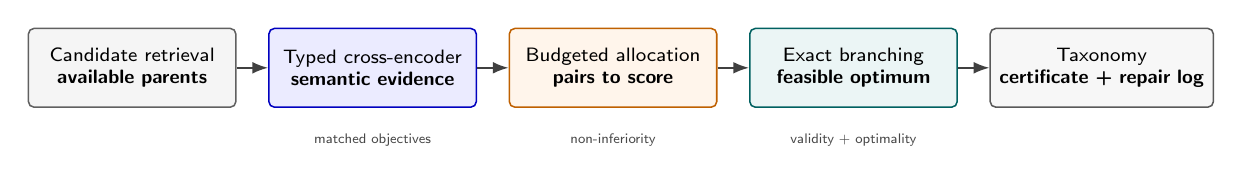
\begin{tikzpicture}[
  font=\sffamily\scriptsize,
  node distance=4mm,
  stage/.style={draw=#1!75!black, fill=#1!8, rounded corners=2pt,
                minimum height=10mm, text width=24mm, align=center, line width=.55pt},
  output/.style={draw=black!65, fill=black!3, rounded corners=2pt,
                 minimum height=10mm, text width=26mm, align=center, line width=.55pt},
  flow/.style={-{Latex[length=2mm]}, line width=.65pt, black!75},
  note/.style={align=center, font=\sffamily\tiny, text=black!72}
]
\node[stage=gray] (retrieve) {Candidate retrieval\\ \textbf{available parents}};
\node[stage=blue, right=of retrieve] (score) {Typed cross-encoder\\ \textbf{semantic evidence}};
\node[stage=orange, right=of score] (allocate) {Budgeted allocation\\ \textbf{pairs to score}};
\node[stage=teal, right=of allocate] (decode) {Exact branching\\ \textbf{feasible optimum}};
\node[output, right=of decode] (output) {Taxonomy\\ \textbf{certificate + repair log}};
\draw[flow] (retrieve) -- (score);
\draw[flow] (score) -- (allocate);
\draw[flow] (allocate) -- (decode);
\draw[flow] (decode) -- (output);
\node[note, below=2mm of score] {matched objectives};
\node[note, below=2mm of allocate] {non-inferiority};
\node[note, below=2mm of decode] {validity + optimality};
\end{tikzpicture}

\caption{\method{} architecture and claim boundaries. Retrieval defines available
candidates; typed scoring supplies local semantic evidence; allocation chooses which
additional pairs to score under a fixed budget; and exact decoding alone certifies
global feasibility. Frozen score and candidate interfaces let each claim be evaluated
without attributing semantic truth to the symbolic layer.}
\label{fig:pipeline}
\end{figure*}

Our contributions follow the three claim boundaries in Figure~\ref{fig:pipeline}.
(1) We define an exact constrained-decoding interface that preserves feasible
independent neural decisions, returns a machine-checkable feasibility certificate
and repair log, and exposes structured max-marginal sensitivity diagnostics. (2) We
establish compute-efficient evidence acquisition with a prespecified \NISeeds{}-retraining
non-inferiority test and exact per-graph budget controls. (3) We isolate
semantic, structural, and compute claims through matched binary, pairwise, and listwise
supervision, shared candidate caches, external transfer, and a controlled
competing-cycle suite. Maximum branching itself is established; our
contribution is the decoding-and-allocation contract around frozen neural
taxonomy scores and its claim-specific evaluation.

\section{Related Work}

\paragraph{Taxonomy induction.}
Taxonomy learning commonly separates relation acquisition from construction.
Hearst patterns provide sparse but interpretable evidence
\citep{hearst-1992-automatic}; shared tasks such as TExEval-2 evaluate the
resulting global hierarchy \citep{bordea-etal-2016-semeval}.  Structured belief
propagation jointly models edges and sibling relations
\citep{bansal-etal-2014-structured}, reinforcement learning directly
optimizes holistic tree metrics \citep{mao-etal-2018-end}, and
ContrastMedium extracts a taxonomy from a noisy linked graph
\citep{faralli-etal-2017-contrastmedium}.  Hyperbolic refinement can relocate
or attach terms in an existing noisy taxonomy \citep{aly-etal-2019-every}.
Graph2Taxo transfers graph structure to unseen domains
\citep{shang-etal-2020-taxonomy}.  The concurrent BoostTaxo preprint combines
language-model agents, hybrid candidate retrieval, structure-aware score
calibration, and maximum arborescence \citep{ling2026boosttaxo}.  We compare only to our frozen-candidate \emph{BoostTaxo-open adaptation};
reported paper numbers remain protocol-separated in
Appendix~\ref{app:boosttaxo-context}. Our setting asks a neural scorer and an exact decoder to
construct a forest under one frozen candidate set.  Unlike score calibration
alone, our decoder returns a machine-checkable feasibility certificate and an itemized
repair trace.

\paragraph{Neural lexical relations.}
Pair classifiers can combine dependency paths with distributional
representations \citep{shwartz-etal-2016-improving}.  We instead train a
cross-encoder with typed supervision: distant ancestors, siblings, and
reversed pairs are not generic negatives, but named alternatives whose
probability can be inspected and penalized.

\paragraph{Backbone and comparison scope.}
DeBERTa-v3-base \citep{he2021deberta} is a fixed encoder, not an architectural
contribution or a claimed taxonomy baseline. To isolate supervision, we retrain
binary, pairwise, listwise, and typed objectives with identical initialization,
inputs, compute, candidates, and decoding. We therefore claim an objective
effect conditional on this backbone, not DeBERTa superiority. A fully crossed
backbone--objective study would instead test generality; end-to-end systems
with different data and inference protocols remain contextual comparisons.

\paragraph{Neuro-symbolic structured prediction.}
Neuro-symbolic systems often use neural models to map language into symbols
and deterministic machinery to execute or constrain them
\citep{liang-etal-2017-neural}.  Domain rules can also guide latent structure
under distribution shift \citep{pryor-etal-2023-using}.  Maximum spanning
arborescences have a long NLP history in dependency parsing
\citep{mcdonald-etal-2005-non}.  We adapt this exact construction to taxonomy
forests and, crucially, measure every decision changed by the symbolic layer.
Our forced-inclusion and forced-exclusion gaps are instances of structured
max-marginals, which have been used for confidence filtering and cascaded
inference \citep{weiss-taskar-2010-structured}; they are also closely related to
reduced-cost and sensitivity analysis for constrained optimization. We do not
claim a new confidence primitive. Our contribution is to expose these familiar
quantities in an auditable taxonomy-decoding interface, connect them to
constraint tension, and test whether they can control neural evidence acquisition
under equal pair budgets.

\section{Problem Formulation}

Let $V$ be the supplied vocabulary. The public edge convention is
$c\!\rightarrow\!p$: child $c$ has direct parent $p$. A candidate generator
returns $C(c)\subseteq V\setminus\{c\}$, and neural modules assign potentials
$s_{cp}$ for $p\in C(c)$ and $r_c$ for the virtual \rootnode. Define
\begin{align}
 \mathcal A_C(c)&=C(c)\cup\{\rootnode\},\\
 \phi_c(q)&=\begin{cases}r_c,&q=\rootnode,\\s_{cq},&q\in C(c).\end{cases}
\end{align}
and let the output be a parent function
$y\in\mathcal Y(C)=\prod_{c\in V}\mathcal A_C(c)$.
For $F_y=\{c\rightarrow y(c):y(c)\neq\rootnode\}$, define
\begin{equation}
 \mathcal F(C)=\{y\in\mathcal Y(C):(V,F_y)\text{ is acyclic}\}.
\end{equation}
Because $y$ is a function, every term has exactly one parent-or-root decision;
omitting root edges yields a rooted forest. Independent decoding chooses the
largest local potential separately and can violate acyclicity. With
$S_\phi(y)=\sum_{c\in V}\phi_c(y(c))$, \method{} instead solves
\begin{equation}
 y^*(C)=\arg\max_{y\in\mathcal F(C)}S_\phi(y).
 \label{eq:objective}
\end{equation}

\section{Method}

\subsection{Role-Conditioned Candidate Retrieval}

We encode labels and available glosses with Qwen3-Embedding-0.6B
\citep{zhang2025qwen3embedding}.  The same encoder receives explicit
\texttt{[CHILD]} and \texttt{[PARENT]} role markers, preventing a symmetric
similarity function from silently treating direction as irrelevant.  Cosine
search supplies the top 50 candidate parents per child; identity edges are
masked.  Candidate caches are frozen and shared by every retraining and decoder, so
all controlled comparisons see identical retrieval evidence.

\subsection{Typed Neural Potentials}

For a candidate pair $(c,p)$, a DeBERTa-v3-base cross-encoder
\citep{he2021deberta} predicts $\pi_z(c,p)=P_\theta(z\mid c,p)$ over five
labels: \textsc{direct}, \textsc{ancestor}, \textsc{sibling},
\textsc{reverse}, and \textsc{unrelated}.
This label space encodes the main ways semantic similarity can be misleading:
\emph{poodle}$\rightarrow$\emph{animal} is related but too distant;
\emph{poodle}$\rightarrow$\emph{spaniel} is a sibling; and
\emph{dog}$\rightarrow$\emph{poodle} reverses direction.  The local edge
potential is
\begin{align}
s_{cp}={}&\log\pi_{\textsc{direct}}(c,p)
-\lambda_a\pi_{\textsc{ancestor}}(c,p)\nonumber\\
&-\lambda_s\pi_{\textsc{sibling}}(c,p)
-\lambda_v\pi_{\textsc{reverse}}(c,p)\nonumber\\
&-\lambda_u\pi_{\textsc{unrelated}}(c,p).
 \label{eq:potential}
\end{align}
The fixed mapping is
$(\lambda_a,\lambda_s,\lambda_v,\lambda_u)=(0.5,0.25,1.0,0.25)$; Section~\ref{sec:ablations}
tests whether they help beyond the learned direct log-probability.

The same encoder has a parent-independent head $r_c$ trained to identify roots
from the child label and definition.  This is a \emph{neural} component: it
models forest segmentation and allows abstention from a poor candidate edge.
Calling root prediction ``symbolic'' would conflate learned evidence with a
hard constraint.

\subsection{Exact Constrained Decoding}

We construct an auxiliary graph in the conventional parent-to-child
orientation.  It contains one node per term plus \rootnode{}, edges
$p\rightarrow c$ with weight $s_{cp}$, and \rootnode$\rightarrow c$ with
weight $r_c$.  An exact Chu--Liu/Edmonds maximum branching
\citep{edmonds1967optimum} selects a spanning arborescence rooted at
\rootnode{}.  Reversing non-root edges returns our child-to-parent forest.
Maximum branching is the known optimizer; our contribution is the auditable
interface around it. The decoder takes frozen neural potentials as input,
returns the maximum-scoring member of the declared feasible family, verifies
the output constraints, and records every changed local decision. These
diagnostics later inform the downstream allocation gate.

\begin{proposition}[Exact-decoding guarantee]
Rooted auxiliary arborescences are in bijection with $\mathcal F(C)$; hence exact
branching returns a maximum-scoring feasible taxonomy. If the unique
independent maxima are already feasible, it preserves every decision.
\end{proposition}
Appendix~\ref{app:projection-proofs} gives the proof and edge-orientation
details.

The proposition makes the symbolic layer auditable: it is inactive unless local
choices conflict globally. Let $\hat y$ be independent decoding. We define
the \emph{constraint tension}
\begin{equation}
T_\phi=S_\phi(\hat y)-S_\phi(y^*)\geq 0.
\label{eq:tension}
\end{equation}
The decoder returns three deliberately separate artifacts: the parent map
$y^*$; a feasibility certificate checked for coverage, one parent-or-root choice,
and acyclicity; and a repair log containing $T_\phi$ and every changed child
with its local potential difference. Global optimality follows from exact
branching and the proposition, and is regression-tested against exhaustive
enumeration on small graphs; the repair log is not presented as an
independently verifiable optimality certificate. Because $S_\phi(\hat y)$ is
constant over feasible alternatives, exact decoding also minimizes
$\sum_c[\phi_c(\hat y(c))-\phi_c(y(c))]$ over $\mathcal F(C)$. A worked
feasibility certificate and proof appear in Appendix~\ref{app:projection-proofs}.

\paragraph{Structured max-marginals.}
Aggregate tension describes the whole repair but does not say whether a
particular selected edge is necessary or how competitive an unselected edge is.
For a selected choice $e\in y^*$ and an unselected feasible choice
$e\notin y^*$, define
\begin{align}
\Delta_e^- &= S_\phi(y^*)-\max_{y\in\mathcal F(C):e\notin y}S_\phi(y),\\
\Delta_e^+ &= S_\phi(y^*)-\max_{y\in\mathcal F(C):e\in y}S_\phi(y).
\label{eq:counterfactual-gaps}
\end{align}
Each inner problem is another exact maximum-branching problem with one choice
forbidden or forced; all other parents are globally re-optimized. Thus these
gaps are forced-exclusion and forced-inclusion structured max-marginals. They
differ from a local top-1--top-2 margin whenever an intervention changes a
cycle or triggers another parent reassignment; the novelty claimed here is
their taxonomy-specific diagnostic and allocation use, not the max-marginal notion.

For evidence allocation we compute the exclusion gap of the selected $k=10$
choice and the inclusion gap of the highest-scoring unselected edge already
inside the scored $k=10$ graph. Consequently the diagnostic needs exact
redecoding but zero extra transformer pairs. A development-only gate combines
these radii with neural uncertainty under the same ranks 11--20 budget as every
control. Their perturbation interpretation, complexity, and audit fields are
detailed in Appendix~\ref{app:projection-proofs}.

\subsection{Budgeted Candidate Scoring}

We first score $k_0=10$ candidates for every child. Neural features summarize
root--edge and top-1--top-2 uncertainty, score level, and the retrieval
boundary. Symbolic features are computed from the local parent graph---cycle
membership and size, fan-in, whether an edge is selected, and its cycle-break
cost. No intermediate exact decode is required. On node-disjoint WordNet
development graphs, let $y_{10}$ and $y_{20}$ be exact decodes at the two
candidate depths. If $e_y(c)$ indicates a correct direct parent (including a
correct \rootnode{} decision) and $a_y(c)$ is child-level ancestor-set F1, the
per-child training target is exactly
\begin{equation}
 q_c=0.25\,[e_{y_{20}}(c)-e_{y_{10}}(c)]
     +[a_{y_{20}}(c)-a_{y_{10}}(c)].
 \label{eq:allocation-target}
\end{equation}
Ridge gates fitted to neural features, symbolic features, or their union rank
children by expected value of additional scoring.

At test time the gate allocates an exact per-graph budget equal to 75\% of
full $k=20$ pairs. Lazy batched scoring evaluates only the selected ranks
11--20, and one final exact decode enforces the unchanged hard
constraints. Neural-only, symbolic-only, random, and uniform
round-robin controls receive exactly the same pair count within every graph.
The scorer, candidate cache, and final decoder are shared, so allocation is
the only manipulated factor. Full $k=20$ is the measured compute reference.
The gate observes only pre-acquisition diagnostics and never changes the
validity predicate or sees test labels. Ranked acquisition returns exactly the same
pair count for every policy, and final decoding always returns a feasible
taxonomy. Appendix~\ref{app:acquisition-proofs} formalizes the acquisition
objective and proves these invariants.


\subsection{Why Sparse Repairs Affect Ancestor F1}

An edge is local, but its transitive consequences are not.  In a forest,
suppose a valid repair reattaches the subtree rooted at $c$ from $p$ to $q$.
Let $D(c)$ include $c$ and its descendants, and $A(v)$ denote $v$ and its
ancestors before the repair.  Every $d\in D(c)$ changes the same upstream
ancestor suffix; the number of ancestor-pair labels flipped is
\begin{equation}
 |D(c)|\bigl(|A(p)\setminus A(q)|+|A(q)\setminus A(p)|\bigr),
 \label{eq:amplification}
\end{equation}
where the valid reattachment requires $q\notin D(c)$.
Thus a decoder may change very few direct-parent decisions yet measurably
alter ancestor F1.  This is a structural amplification effect, not evidence
that symbolic inference discovered new lexical candidates.

\section{Experimental Design}

Our experiments test three questions. \textbf{Semantic evidence}: does typed
supervision improve direct-parent selection under matched backbone, candidate
pool, and pair-encoding budget? \textbf{Structural feasibility}: after scores
are frozen, does exact decoding guarantee feasibility and attain the constrained optimum?
\textbf{Compute efficiency}: can a 75\%-pair allocation remain within
prespecified edge and ancestor margins of full scoring? Candidate ceilings,
external transfer, and decision-level sensitivity diagnostics are supporting analyses.
This ordering prevents an end-to-end gain from being credited wholesale to
``symbolic reasoning.''

\subsection{Data and Decontamination}

We train on WordNet 3.0 \citep{miller1995wordnet} and evaluate in two settings.
The external benchmark is the six English TExEval-2 taxonomies
\citep{bordea-etal-2016-semeval}.  Our primary \textsc{Macro4} average uses
Science, Science-EuroVoc, Environment-EuroVoc, and Food. Results for the two
WordNet-derived TExEval domains are confined to the supplement. The second
benchmark consists of 243 held-out WordNet subgraphs
drawn from lexical domains excluded from training. Thus evaluation combines
complete external vocabularies with a larger node-disjoint ontology split.

Before generating relation examples, we normalize case, whitespace, hyphens,
and underscores, then remove every WordNet synset with any lemma occurring in
TExEval-2 or the frozen Schema.org validation vocabulary.  This removes 4,745
synsets.  The build audit reports zero remaining external-synset overlap and
zero synset overlap among train, development, and test.  Ancestor and sibling
labels are generated only within a split, so no cross-split path is traversed.
After filtering, training contains 71,308 synsets, 399,228 relation examples,
and 71,308 node-level root examples (8,142 positive).
This audit controls task-specific supervision and split construction; it cannot
establish absence from the undocumented pretraining corpora of DeBERTa, the
embedding retriever, or the generative Qwen models. We use ``decontaminated''
only in the former, directly auditable sense.
A post-freeze input audit on node-disjoint WordNet further drops \ef{} from
\InputFull{} with labels and glosses to \InputLabels{} with labels only,
\InputDefinitions{} with glosses only, and \InputAnonymous{} after replacing
labels by stable opaque identifiers (Appendix Table~\ref{tab:input-controls}). This does
not audit pretraining, but argues against simple label lookup as the explanation.

\begin{table}[t]
\centering
\small
\setlength{\tabcolsep}{3.5pt}
\begin{tabular}{lrrrr}
\toprule
Domain & Nodes & Edges & R@20 & R@50\\
\midrule
Science & 452 & 465 & 79.35 & 92.04\\
Science-EuroVoc & 125 & 124 & 98.39 & 100.00\\
Env.-EuroVoc & 261 & 261 & 69.35 & 80.08\\
Food & 1,556 & 1,587 & 29.11 & 36.17\\
\midrule
Macro4 & -- & -- & 69.05 & 77.07\\
\bottomrule
\end{tabular}
\caption{External data sizes and candidate edge recall (\%). Recall uses all
gold edges as denominator; missing gold parents therefore remain misses.}
\label{tab:retrieval}
\end{table}

Table~\ref{tab:retrieval} exposes a major ceiling: Food candidate recall is
only 36.17 even at 50 candidates.  No downstream scorer or constraint can
recover an absent gold parent.  We therefore separate retrieval failure (gold
missing), neural scoring failure (gold available but not selected), and
structural inference failure (local choices are jointly infeasible).

\begin{proposition}[Candidate-omission ceiling]
Let $E^*$ be the gold edges and $E_C=\{(c,p):p\in C(c)\}$ the retrieved
candidate edges. Every decoder restricted to $E_C$ satisfies
\begin{equation}
\operatorname{Recall}_{\rm edge}(y)\leq
\frac{|E^*\cap E_C|}{|E^*|}.
\label{eq:oracle-bound}
\end{equation}
\end{proposition}
\begin{proof}
No predicted true positive can lie outside $E^*\cap E_C$.
\end{proof}

This bound makes retrieval recall part of the evaluation, not an implementation
detail. Together with non-interference, it explains why the primary semantic
movement can be modest: symbols can certify feasibility over supplied
candidates and allocate more scoring, but cannot recover a parent that
retrieval omitted.

\subsection{Training and Selection}

The cross-encoder is trained for at most three epochs with batch size 32,
learning rate $2\times10^{-5}$, linear warmup over 6\% of steps, gradient norm
1, and FP32 master weights with BF16 autocast.  Early stopping monitors
development macro-F1 with patience 2 and $10^{-4}$ minimum improvement; only
the best checkpoint is evaluated. The relation development macro-F1 over five
development retrainings is $91.17\pm0.31$. Root temperature/bias and optional
decoder policies are selected only on node-disjoint WordNet development data.

Evidence partitions are not pooled. Development retrainings select model and
calibration choices; five fresh retrainings (IDs 47--51) evaluate component decomposition,
ten further retrainings (IDs 117--126) compare supervision objectives, and 30 disjoint
retrainings (IDs 87--116) test non-inferiority. Here IDs denote random
initialization identifiers; the statistical unit is the independently trained model. The matched objectives share the backbone,
pair budget, encodings per update, optimizer-update count, and scheduler. Each
analysis fixes its inputs, contrasts, and reporting rule before inspecting its
outputs; Appendix~\ref{app:provenance} gives complete retraining provenance.

\subsection{Metrics and Baselines}

We report direct edge F1 (\ef), transitive ancestor F1 (\af), and structural
validity. A decoded output is valid iff $y\in\mathcal F(C)$: it covers every
supplied node with exactly one parent-or-root choice and its non-root edges are
acyclic. Repair statistics count changed child decisions and constraint
tension. For the component
decomposition we use 10,000 paired child-level bootstrap samples; its
five-retraining estimates are descriptive. For the headline matched semantic
contrasts, ten independent retrainings are the sampling unit and 100,000 paired
bootstrap draws form two-sided 95\% intervals. The allocation evaluation uses
30 independent retrainings and prespecified paired,
one-sided Student-$t$ lower bounds. Non-inferiority requires both lower bounds
to exceed the declared margins of $-0.5$ \ef{} and $-1.0$ \af{} points, an
intersection--union decision rather than a failure-to-reject argument.
We isolate measured combined and full-$k=20$ pipelines after warmup and report
scored pairs, CUDA time, wall time, throughput, and peak memory. Test labels
never select a gate, control, or margin.

The three matched alternatives use the same pretrained DeBERTa backbone,
retrieved pool, pair representation, \MatchedObjectivePairEncodings{} transformer pair
encodings per epoch, \MatchedObjectivePairsPerUpdate{} encodings per update,
\MatchedObjectiveUpdates{} optimizer updates per epoch, scheduler, epochs, early stopping,
random initializations, learned root model, and exact decoder as \method{}.
The balanced binary objective predicts direct-parent versus not-direct; the
pairwise objective ranks each direct parent against a matched hard negative;
the listwise objective contrasts it with two unique hard negatives in each
size-\RobustListwiseGroupSize{} group. Objective-specific batch item counts
are chosen so every update encodes the same number of pairs. Thus the typed row
changes supervision, not backbone, candidate access, pair budget, update count,
or schedule. Graph2Taxo, Qwen rerankers, and the disclosed BoostTaxo-open
adaptation use different training or inference protocols and therefore serve
as supporting context only (Appendix~\ref{app:full-results}).

\section{Results}

Unless a controlled comparison is named, \method{} denotes the typed scorer,
learned root potential, exact constrained decoder, and top-50 retrieval. Across
five independent evaluation retrainings, this reference configuration obtains
38.07 \ef{}, 40.87 \af{}, and 100\% validity on TExEval-2 Macro4. Each table
below estimates a distinct contrast; estimates from different retraining sets
are not pooled.

\subsection{Component Decomposition}


\begin{table*}[t]
\centering
\small
\begin{tabular}{lcccccc}
\toprule
& \multicolumn{3}{c}{TExEval-2 Macro4} & \multicolumn{3}{c}{Node-disjoint WordNet}\\
\cmidrule(lr){2-4}\cmidrule(lr){5-7}
System & \ef & \af & Valid & \ef & \af & Valid\\
\midrule
Embedding top-1 & 17.57$\pm$0.00 & 12.32$\pm$0.00 & 0.0 & 10.95$\pm$0.00 & 9.47$\pm$0.00 & 0.0\\
Typed relation top-1 & 38.46$\pm$1.84 & 36.76$\pm$1.74 & 0.0 & 60.00$\pm$0.77 & 60.05$\pm$0.81 & 0.0\\
$+$ learned \rootnode{} & 38.05$\pm$1.91 & 40.25$\pm$4.42 & 60.0 & 63.93$\pm$0.70 & 68.65$\pm$0.25 & 98.68\\
$+$ exact branching & 38.07$\pm$1.90 & 40.87$\pm$3.96 & 100.0 & 63.93$\pm$0.71 & 68.66$\pm$0.24 & 100.0\\
\bottomrule
\end{tabular}
\caption{Five independent evaluation retrainings. F1 and validity are percentages. Macro4
excludes two WordNet-derived TExEval domains; the second benchmark is node- and
lexical-domain-disjoint. All rows use the same candidate caches.}
\label{tab:main}
\end{table*}

As Table~\ref{tab:main} shows, typed relation supervision is the largest source
of local accuracy: it raises
Macro4 \ef{} from 17.57 to 38.46.  This supports explicitly distinguishing a
direct parent from nearby but wrong relation types.  Independent root modeling
trades 0.41 \ef{} for 3.49 \af{} points on external domains and raises both
metrics strongly on node-disjoint WordNet.  However, it is not a structural
guarantee: only 60\% of external retraining-level domain averages and 98.68\% of
WordNet subgraphs are valid.

Exact branching raises validity to 100\% on both benchmarks; this is the
primary symbolic-inference claim. Relative to independent root-aware choices, it
changes Macro4 \ef{} by +0.02 and \af{} by +0.62 points. The small local
delta is a non-interference property: the decoder certifies feasibility while
preserving compatible neural decisions, rather than acting as an uncontrolled
semantic reranker.
The node-disjoint result also shows that the guarantee is not tied to the
external benchmark: \ef/\af{} are 63.93/68.66 with complete validity.

\subsection{Matched Semantic Evidence}

\begin{table*}[t]
\centering
\small
\begin{tabular}{lrrrr}
\toprule
& \multicolumn{2}{c}{TExEval-2 Macro4} & \multicolumn{2}{c}{Schema.org}\\
\cmidrule(lr){2-3}\cmidrule(lr){4-5}
Objective & \ef & \af & \ef & \af\\
\midrule
Balanced binary & \MatchedObjectiveTexevalBinaryEdge & \MatchedObjectiveTexevalBinaryAncestor & \MatchedObjectiveSchemaBinaryEdge & \MatchedObjectiveSchemaBinaryAncestor\\
Pairwise & \MatchedObjectiveTexevalPairwiseEdge & \MatchedObjectiveTexevalPairwiseAncestor & \MatchedObjectiveSchemaPairwiseEdge & \MatchedObjectiveSchemaPairwiseAncestor\\
Listwise & \MatchedObjectiveTexevalListwiseEdge & \MatchedObjectiveTexevalListwiseAncestor & \MatchedObjectiveSchemaListwiseEdge & \MatchedObjectiveSchemaListwiseAncestor\\
Typed & \textbf{\MatchedObjectiveTexevalTypedEdge} & \textbf{\MatchedObjectiveTexevalTypedAncestor} & \textbf{\MatchedObjectiveSchemaTypedEdge} & \textbf{\MatchedObjectiveSchemaTypedAncestor}\\
\bottomrule
\end{tabular}
\caption{Ten independent matched retrainings (mean$\pm$SD, percent).
All rows use the same backbone, candidates, exact pair-encoding budget,
\MatchedObjectivePairsPerUpdate{} encoded pairs per update, \MatchedObjectiveUpdates{} optimizer
updates per epoch, learned root model, and exact decoder; only the supervision
objective changes. Every decoded output is valid.}
\label{tab:matched-supervision}
\end{table*}

Table~\ref{tab:matched-supervision} shows that typed supervision exceeds the
balanced binary control by
\MatchedObjectiveTexevalTypedMinusBinaryEdge{} \ef{} points (paired 95\% CI across retrainings
[\MatchedObjectiveTexevalTypedMinusBinaryEdgeLow, \MatchedObjectiveTexevalTypedMinusBinaryEdgeHigh]) and
\MatchedObjectiveTexevalTypedMinusBinaryAncestor{} \af{} points
([\MatchedObjectiveTexevalTypedMinusBinaryAncestorLow, \MatchedObjectiveTexevalTypedMinusBinaryAncestorHigh]).
Against pairwise ranking, the gains are
\MatchedObjectiveTexevalTypedMinusPairwiseEdge/\MatchedObjectiveTexevalTypedMinusPairwiseAncestor{}
\ef/\af{} points; against the strongest listwise control they are
\MatchedObjectiveTexevalTypedMinusListwiseEdge/\MatchedObjectiveTexevalTypedMinusListwiseAncestor{}
points, with intervals
[\MatchedObjectiveTexevalTypedMinusListwiseEdgeLow,\MatchedObjectiveTexevalTypedMinusListwiseEdgeHigh]/
[\MatchedObjectiveTexevalTypedMinusListwiseAncestorLow,\MatchedObjectiveTexevalTypedMinusListwiseAncestorHigh].
All six TExEval intervals exclude zero. These controls support the value of typed
relation supervision under exactly matched capacity and update budget; unmatched Graph2Taxo,
Qwen, and BoostTaxo-open comparisons remain contextual
(Appendix~\ref{app:full-results}).
The advantage transfers to Schema.org under the same label-free top-200
candidate pool and exact decoder: typed supervision exceeds balanced binary
training by \MatchedObjectiveSchemaTypedMinusBinaryEdge/\MatchedObjectiveSchemaTypedMinusBinaryAncestor{}
\ef/\af{} points and pairwise ranking by
\MatchedObjectiveSchemaTypedMinusPairwiseEdge/\MatchedObjectiveSchemaTypedMinusPairwiseAncestor{} points;
all paired 95\% intervals across retrainings exclude zero.
A post-hoc multiplicity sensitivity over the ten core
matched endpoints---all six TExEval contrasts and the four Schema binary/pairwise
contrasts---every studentized-bootstrap simultaneous interval remains above
zero (minimum lower bound \MatchedObjectiveMatchedCoreMinLower{} points), and all
Holm-adjusted exact sign-flip $p$-values are below .05.

\subsection{Feasibility and Optimality}

Exact constrained decoding modifies only 42 of 22,535 decisions yet makes every
output valid; across four frozen scorers it raises validity to 100\% while
activation frequency varies by scorer. Constraint tension is almost perfectly
associated with edit rate ($\rho=\TensionChangeRho$) and cyclic-node rate
($\rho=0.99$), making each intervention auditable. Decision-level changes,
task-metric intervals, and examples are in Appendix Table~\ref{tab:repair}.

A prespecified competing-cycle suite tests the regime in which the
constraint layer is deliberately active rather than nearly non-interfering.
Across \PressureRuns{} synthetic trials in \PressureCells{} cells, exact decoding
remains \PressureExactValid\% valid with zero optimality gap. For a feasible
decoder $m$, define $G_m=S_\phi(y^*)-S_\phi(y_m)\geq0$. Greedy and
lexicographic minimal-edit repair incur mean gaps
\PressureGreedyRegret{} and \PressureMinimalRegret{}; on overlapping competing
cycles these rise to \PressureOverlapGreedyRegret{} and
\PressureOverlapMinimalRegret{}, whereas $G_{\rm exact}=0$. Full details
and runtime are reported in Appendix~\ref{app:constraint-pressure-v2}.

Exhaustive enumeration on \RobustSolverTrials{} small graphs independently
matches every exact optimum (maximum score gap \RobustSolverMaxGap{}). Under an
equal \CertPairFraction\% budget, global gaps also improve over random by
\CertOnlyMinusRandomEdge{} \ef{} and over uniform allocation by
\CertOnlyMinusUniformAncestor{} \af{} points; full intervals and controls are
in Appendix Table~\ref{tab:certificate-allocation}.

\subsection{Failure Attribution}

The decoder cannot recover a gold parent outside the candidate set: Food recall
is only 36.17\% even at $k=50$. We therefore attribute missing candidates,
misranking, and infeasible local choices separately. Full ceilings are in
Appendix~\ref{app:additional-diagnostics}, and the multi-parent analysis is in
Appendices~\ref{app:multiparent-dag} and~\ref{app:family-selection}.

\subsection{Independent Transfer}

On MAG-PSY, typed supervision improves MRR/accuracy over balanced binary by
\MatchedObjectiveMAGPSYTypedMinusBinaryMRR{}/\MatchedObjectiveMAGPSYTypedMinusBinaryAcc{}, over
pairwise by \MatchedObjectiveMAGPSYTypedMinusPairwiseMRR{}/
\MatchedObjectiveMAGPSYTypedMinusPairwiseAcc{}, and over listwise by
\MatchedObjectiveMAGPSYTypedMinusListwiseMRR{}/\MatchedObjectiveMAGPSYTypedMinusListwiseAcc{}.
All six paired 95\% intervals exclude zero. A post-hoc six-endpoint
simultaneous-bootstrap sensitivity analysis is wholly positive (smallest lower
bound \MatchedObjectiveMAGPSYMinLower{}), and every Holm-adjusted $p<.05$. The complete
table and node-disjoint noun/verb transfer are in
Appendix Table~\ref{tab:transfer}.

\subsection{Compute Non-Inferiority}
\label{sec:adaptive-confirmatory}

\begin{table}[t]
\centering
\small
\setlength{\tabcolsep}{3pt}
\begin{tabular}{lrrrrr}
\toprule
Policy & \ef & \af & Pairs & GPU & Wall\\
\midrule
Combined & \NICombinedEdge & \NICombinedAncestor & 75\% &
$-\NIGPUSaving$\% & $-\NIWallSaving$\%\\
Full $k=20$ & \NIFullEdge & \NIFullAncestor & 100\% & ref. & ref.\\
\bottomrule
\end{tabular}
\caption{Thirty-retraining non-inferiority evaluation over four fixed domains
(Macro4, percent).
Compute columns are paired savings relative to full scoring; every output is
structurally valid.}
\label{tab:voc-confirmatory}
\end{table}

As Table~\ref{tab:voc-confirmatory} shows, at 75\% of the pair budget, combined
differs from full scoring by
\NIEdgeDiff{} \ef{} and \NIAncestorDiff{} \af{} points. The prespecified
one-sided lower bounds are \NIEdgeLower{} and \NIAncestorLower{}, both above
their respective $-\NIEdgeMargin$ and $-\NIAncestorMargin$ margins. The
intersection--union test therefore establishes non-inferiority on both
endpoints across \NISeeds{} independent retrainings. This is an affirmative margin
test, not an inference from a non-significant difference.

The margins correspond to 1.31\% and 2.86\% of the full system's edge and
ancestor F1. A sensitivity grid and leave-one-domain-out audit preserve the
declared decision and are reported in Appendix~\ref{app:allocation-audits}.

The reduced policy evaluates \NIPairSaving\% fewer pairs and saves
\NIGPUSaving\% CUDA time and \NIWallSaving\% wall time. Against the
equal-budget neural-only gate, its structural features add
\NIMinusNeuralEdge{} \ef{} points (95\% CI
[\NIMinusNeuralEdgeLow, \NIMinusNeuralEdgeHigh]), providing a replicated
edge gain. Earlier independent evidence and all equal-budget controls are
reported in Appendix~\ref{app:allocation-audits}.


\section{Conclusion}

\method{} separates three claims that are often conflated. Under matched
backbone, candidate access, pair encodings, optimizer updates, and scheduler,
typed supervision improves both semantic endpoints over balanced binary,
pairwise, and listwise objectives on TExEval-2. The same matched protocol
replicates against binary and pairwise controls on Schema.org and against all
three objectives on MAG-PSY. Exact constrained decoding then guarantees
feasibility and attains the constrained score optimum; across 1,280
competing-cycle trials it remains 100\% valid with zero optimality gap. Finally,
a prespecified 30-retraining test establishes that the 75\% pair-budget policy is
non-inferior to full scoring within 0.5 \ef{} and 1.0 \af{} points while saving
\NIGPUSaving/\NIWallSaving\% GPU/wall time. Schema.org, MAG-PSY, and
node-disjoint WordNet noun/verb evaluation extend the matched evidence beyond
the four TExEval domains. Exact counterfactual gaps additionally form a useful
standalone allocation signal under equal budgets.

\section*{Limitations}

\paragraph{Comparison scope.}
All matched objectives use DeBERTa-v3-base. This deliberate control isolates
supervision, but establishes neither encoder superiority nor
backbone-independent gains. A fully crossed backbone--objective replication is
needed for that claim. Likewise, published end-to-end systems use different
training data, candidate access, or enrichment protocols. We therefore lack a
contemporary protocol-compatible end-to-end baseline and make no
state-of-the-art claim; those systems provide context only.

\paragraph{Structural scope.}
On the natural benchmarks, exact decoding changes only 42 of 22,535 local
decisions because most independent predictions are already feasible. Its main
empirical role is consequently deterministic validity rather than a large
semantic gain; the controlled cycle suite tests behavior when constraints are
active. The decoder also cannot recover an omitted candidate or
guarantee semantic truth. The primary output has one parent per term, while the
supplementary two-parent analysis establishes feasibility for DAGs rather than
reliable variable-cardinality recovery.

\paragraph{Statistical and protocol scope.}
The 30 independent retrainings are over four fixed benchmarks, not samples
of 30 new domains, and the non-inferiority margins remain an application
judgment. Protocol files were hash-locked before results were produced. Before
outcome inspection, an eligibility check was corrected without changing
training, checkpoints, candidates, decoding, or metrics; this auditable record
is still weaker than a public, independently timestamped preregistration. Finally, all
resources are English, and undocumented model pretraining corpora cannot be
fully audited. Multilingual and larger production taxonomies remain future
work.

\section*{Ethical Considerations}

Automatically induced taxonomies can encode lexical and social biases from
their pretrained models and source resources.  Structural validity does not
make a hierarchy fair, complete, or suitable for consequential use.  Systems
should retain source evidence and repair logs and should be reviewed by
domain experts before deployment.  Our data consist of public lexical and
taxonomy resources and do not contain personal data.  We report model names,
data versions, decontamination rules, compute configuration, and negative
ablations to reduce misleading reuse.

\bibliography{references,family_references}

\appendix

\section{Proof Detail and Edge Orientation}
\label{app:projection-proofs}

\paragraph{Exact-decoding guarantee.}
Each non-root node in a rooted auxiliary arborescence has exactly one incoming
edge, so every term selects one vocabulary parent or \rootnode{}; deleting the
virtual root cannot create a cycle. Conversely, reverse every taxonomy edge
and add \rootnode$\rightarrow c$ for each forest root. The result is a rooted
spanning arborescence with the same score, proving the bijection. Because
Chu--Liu/Edmonds maximizes that score, mapping its optimum back proves validity
and optimality. If unique independent maxima are feasible, their summed local
maxima upper-bound every assignment and attain that bound, so exact decoding
preserves them.

\paragraph{Constraint tension and worked repair log.}
The term $S_\phi(\hat y)$ is constant in $y$, hence minimizing
$\sum_c[\phi_c(\hat y(c))-\phi_c(y(c))]$ over $\mathcal F(C)$ is exactly
maximizing $S_\phi(y)$. Suppose the independent choices are
\emph{dog}$\rightarrow$\emph{animal} (3.0),
\emph{animal}$\rightarrow$\emph{organism} (2.8), and
\emph{organism}$\rightarrow$\emph{dog} (2.7), forming a cycle, while their
root potentials are 0.5, 0.7, and 2.2. Exact decoding changes only
\emph{organism}$\rightarrow$\rootnode{} and returns tension $2.7-2.2=0.5$;
the alternative breaks cost 2.1 and 2.5.

\paragraph{Counterfactual radius.}
Changing only choice $e$ shifts every feasible solution containing it equally
and leaves all excluding solutions unchanged. Therefore the forced-exclusion
or forced-inclusion optimum crosses the unconstrained optimum exactly at
$\Delta_e^-$ or $\Delta_e^+$ in Equation~\ref{eq:counterfactual-gaps}; equality
permits a tie. With $k$ candidates, the graph has $|V|+1$ nodes and at most
$(k+1)|V|$ edges. We persist the selected parent, potential, local-argmax
change, and implicated cycle/root decision.

Our files expose child-to-parent edges because this is convenient for taxonomy
evaluation.  The branching implementation reverses them internally, runs
maximum branching in parent-to-child orientation, and reverses selected
non-root edges on return.  Self-loops and candidates outside the supplied
vocabulary are removed.  A lexicographic cardinality constant first maximizes
edge count in the numerical implementation; all spanning arborescences have
the same edge count, so their ordering by the original objective is unchanged.

For Equation~\ref{eq:amplification}, unique parent paths imply that every
descendant of $c$ shares its upstream suffix.  Replacing $c\rightarrow p$ by
$c\rightarrow q$ removes precisely the non-common members of $A(p)$ and adds
the non-common members of $A(q)$ for every $d\in D(c)$.  Multiplication by
$|D(c)|$ gives the number of flipped ordered ancestor pairs.  The equation
assumes a valid reattachment that does not place $q$ inside $D(c)$.
\section{Acquisition Proofs and Sensitivity}
\label{app:acquisition-proofs}

Let $C_0(c)$ be the scored prefix, $U_c$ the available unscored pairs for
child $c$, and $m_c=|U_c|$. For an acquisition set
$A\subseteq\bigcup_c U_c$, define $b_c(A)=|A\cap U_c|$ and
$C_A(c)=C_0(c)\cup(A\cap U_c)$. For frozen potentials,
\begin{equation}
 y^*(A)=\arg\max_{y\in\mathcal F(C_A)} S_\phi(y).
 \label{eq:acquisition-decode}
\end{equation}
The gate fits $\widehat q_c$ to the development-only target in
Equation~\ref{eq:allocation-target} and orders acquisitions by the explicit
surrogate
\begin{equation}
 \widetilde Q(A)=\sum_{c:m_c>0}\widehat q_c\,\frac{b_c(A)}{m_c},
 \qquad |A|=B.
 \label{eq:acquisition}
\end{equation}
Test labels are unavailable to the fitted gate and all allocation decisions.

\paragraph{Exact budget.}
For each child, enumerate its available ranks $k_0+1,\ldots,k_{\max}$.
Concatenating these finite lists in any policy-defined child order produces an
ordered list of all available extra pairs. Taking its first $B$ elements
therefore returns exactly $B$ distinct pairs whenever the list has length at
least $B$. Random, uniform, neural, symbolic, residual, and permutation
controls differ only in this order. Our audit checks equality within every
retraining--graph cell rather than inferring it from a global average.

\paragraph{Score monotonicity.}
If $A\subseteq A'$, then $C_A(c)\subseteq C_{A'}(c)$ for every child and
$\mathcal F(C_A)\subseteq\mathcal F(C_{A'})$. Hence
\[
 \max_{y\in\mathcal F(C_{A'})}S_\phi(y)
 \geq \max_{y\in\mathcal F(C_A)}S_\phi(y).
\]
This concerns only the frozen model score. A newly available high-scoring
false edge can increase that score while decreasing semantic F1, so we report
model-score and task metrics separately.

\paragraph{One-edge exchange diagnostic.}
Fix the exact base solution $y^*$ and all decisions except child $c$. Let
$\mathcal A_c(y^*_{-c})$ contain the parents (including \rootnode{}) that
preserve feasibility under this single substitution, and define
\[
 \gamma_c=\phi_c(y^*(c))-\max_{q\in\mathcal A_c(y^*_{-c})
 \setminus\{y^*(c)\}}\phi_c(q)\geq0.
\]
If every local potential for $c$ changes by at most $\epsilon$ and
$\gamma_c>2\epsilon$, the selected parent remains optimal among all such
one-edge exchanges: the gap can shrink by at most $2\epsilon$. This identifies
locally fragile decisions, but does not rule out coordinated multi-edge
exchanges and is not a full reduced cost for Edmonds' algorithm.

\paragraph{Cost.}
With $n=|V|$ and prefix width $k_0$, neural prefix scoring uses $O(nk_0)$
pairs, gate ranking costs $O(n\log n)$, and lazy scoring adds exactly $B$
pairs. The optional sensitivity diagnostic and final decode each invoke a
polynomial-time maximum branching; all equal-budget controls reuse their
score tensors. We report measured wall/CUDA time because these asymptotic
statements do not capture transformer batching or data movement.

\section{Full Pooled Results}
\label{app:full-results}

\begin{table}[h]
\centering
\scriptsize
\setlength{\tabcolsep}{3pt}
\begin{tabular}{llrr}
\toprule
Benchmark & Objective & MRR & Acc@1\\
\midrule
MAG-PSY & balanced binary & \MatchedObjectiveMAGPSYBinaryMRR & \MatchedObjectiveMAGPSYBinaryAcc\\
        & pairwise & \MatchedObjectiveMAGPSYPairwiseMRR & \MatchedObjectiveMAGPSYPairwiseAcc\\
        & listwise & \MatchedObjectiveMAGPSYListwiseMRR & \MatchedObjectiveMAGPSYListwiseAcc\\
        & typed & \textbf{\MatchedObjectiveMAGPSYTypedMRR} & \textbf{\MatchedObjectiveMAGPSYTypedAcc}\\
\bottomrule
\end{tabular}
\caption{Independent matched transfer, retraining IDs 117--126 (mean$\pm$SD), under
the same backbone, data, pair encodings, optimizer updates, and scheduler.}
\label{tab:transfer}
\end{table}

On node-disjoint WordNet noun and verb benchmarks, typed supervision also
exceeds binary and pairwise objectives on MRR and accuracy; the smallest paired
gain is noun MRR versus pairwise,
\MatchedObjectiveNounTypedMinusPairwiseMRR{} (95\% CI
[\MatchedObjectiveNounTypedMinusPairwiseMRRLow{},
\MatchedObjectiveNounTypedMinusPairwiseMRRHigh{}]).

The pooled retraining IDs 42--51 give 38.41$\pm$2.21 Macro4 \ef{},
41.60$\pm$3.98 Macro4 \af{}, and 100\% validity for plain exact branching.
On node-disjoint WordNet, the corresponding results are
63.36$\pm$0.91 \ef{}, 68.40$\pm$0.36 \af{}, and 100\% validity.  We keep these
as secondary evidence because retraining IDs 42--46 informed model development.

\begin{table*}[h]
\centering
\small
\setlength{\tabcolsep}{5pt}
\begin{tabular}{llcccc}
\toprule
System & Neural evidence & $k$ & \ef & \af & Valid\\
\midrule
Embedding top-1 & none & 50 & 17.57 & 12.32 & 0\\
Binary DeBERTa + exact & binary pairs & 50 & \BinaryEdge & \BinaryAncestor & 100\\
Graph2Taxo \citep{shang-etal-2020-taxonomy} & graph objective & own & \GraphEdge & \GraphAncestor & 100\\
\method{}@20 + exact & typed pairs & 20 & \TaxoTwentyEdge & \TaxoTwentyAncestor & 100\\
Qwen3-8B + exact & zero-shot pairs & 20 & \QwenEightEdge & \QwenEightAncestor & 100\\
Qwen3.5-27B + exact & zero-shot pairs & 20 & \QwenLargeEdge & \QwenLargeAncestor & 100\\
BoostTaxo-open + exact & adapted 27B & 20 & \BoostOpenEdge & \BoostOpenAncestor & 100\\
\method{} + exact & typed pairs & 50 & 38.07$\pm$1.90 & 40.87$\pm$3.96 & 100\\
\bottomrule
\end{tabular}
\caption{Contextual Macro4 evaluation (percent). Protocols, training data, and
candidate budgets differ across groups; this table is not used for a matched
state-of-the-art claim. BoostTaxo-open is a disclosed adaptation.}
\label{tab:unified}
\end{table*}

\paragraph{Schema.org controls and candidate-pruning audit.}
The paired 95\% CIs across retrainings for typed minus balanced binary are
[\SchemaTransferSchemaTypedMinusBinaryEdgeLow, \SchemaTransferSchemaTypedMinusBinaryEdgeHigh] for
\ef{} and [\SchemaTransferSchemaTypedMinusBinaryAncestorLow,
\SchemaTransferSchemaTypedMinusBinaryAncestorHigh] for \af{}; against pairwise ranking they
are [\SchemaTransferSchemaTypedMinusPairwiseEdgeLow, \SchemaTransferSchemaTypedMinusPairwiseEdgeHigh]
and [\SchemaTransferSchemaTypedMinusPairwiseAncestorLow,
\SchemaTransferSchemaTypedMinusPairwiseAncestorHigh], respectively.
Against listwise, the corresponding mean gaps are
\RobustSchemaTypedMinusListwiseEdge{} and
\RobustSchemaTypedMinusListwiseAncestor{} points, with marginal intervals
[\RobustSchemaTypedMinusListwiseEdgeLow,
\RobustSchemaTypedMinusListwiseEdgeHigh] and
[\RobustSchemaTypedMinusListwiseAncestorLow,
\RobustSchemaTypedMinusListwiseAncestorHigh].
The all-pairs lexical exact control yields \SchemaLexicalEdge{} \ef{} and
\SchemaLexicalAncestor{} \af{}. As a post-hoc secondary contrast, the
label-free top-200 candidate pool reduces pair evaluations from
\SchemaTransferSchemaAllPairs{} to \SchemaTransferSchemaTopPairs{} ($-\SchemaTransferSchemaPairSaving\%$) relative
to typed all-pairs decoding. With the same typed checkpoints, top-200 decoding
changes \ef{} by \SchemaTransferTopVsAllEdge{} points (post-hoc paired-retraining 95\% CI
[\SchemaTransferTopVsAllEdgeLow, \SchemaTransferTopVsAllEdgeHigh]) and \af{} by
\SchemaTransferTopVsAllAncestor{} points
([\SchemaTransferTopVsAllAncestorLow, \SchemaTransferTopVsAllAncestorHigh]), while retaining
\SchemaTransferSchemaValid\% validity. Candidate construction uses no test labels; the
top-200 versus all-pairs comparison itself was specified post hoc and is not a
primary claim.

\begin{table}[h]
\centering
\scriptsize
\setlength{\tabcolsep}{3pt}
\begin{tabular}{llcc}
\toprule
Data & Contrast & \ef{} joint CI & \af{} joint CI\\
\midrule
TExEval-2 & typed $-$ binary & [\RobustTexevalTypedMinusBalancedBinaryEdgeFOneLow, \RobustTexevalTypedMinusBalancedBinaryEdgeFOneHigh] & [\RobustTexevalTypedMinusBalancedBinaryAncestorFOneLow, \RobustTexevalTypedMinusBalancedBinaryAncestorFOneHigh]\\
TExEval-2 & typed $-$ pairwise & [\RobustTexevalTypedMinusPairwiseEdgeFOneLow, \RobustTexevalTypedMinusPairwiseEdgeFOneHigh] & [\RobustTexevalTypedMinusPairwiseAncestorFOneLow, \RobustTexevalTypedMinusPairwiseAncestorFOneHigh]\\
Schema.org & typed $-$ binary & [\RobustSchemaorgTypedMinusBalancedBinaryEdgeFOneLow, \RobustSchemaorgTypedMinusBalancedBinaryEdgeFOneHigh] & [\RobustSchemaorgTypedMinusBalancedBinaryAncestorFOneLow, \RobustSchemaorgTypedMinusBalancedBinaryAncestorFOneHigh]\\
Schema.org & typed $-$ pairwise & [\RobustSchemaorgTypedMinusPairwiseEdgeFOneLow, \RobustSchemaorgTypedMinusPairwiseEdgeFOneHigh] & [\RobustSchemaorgTypedMinusPairwiseAncestorFOneLow, \RobustSchemaorgTypedMinusPairwiseAncestorFOneHigh]\\
\bottomrule
\end{tabular}
\caption{Post-hoc familywise sensitivity over all eight matched endpoints.
Intervals are joint studentized bootstrap intervals over paired retrainings; all
Holm-adjusted exact sign-flip $p$-values are below .05.}
\label{tab:joint-multiplicity}
\end{table}

\subsection{Matched Listwise Robustness}
\label{app:listwise-audit}

The listwise objective ranks one direct parent against two unique hard
negatives while preserving the same backbone, candidates, decoder, and
\RobustListwisePairEncodings{} transformer pair encodings per epoch. It is a
competitive control rather than a strawman: on TExEval-2 it exceeds pairwise
by \RobustTexevalListwiseMinusPairwiseEdge{} \ef{} (95\% CI
[\RobustTexevalListwiseMinusPairwiseEdgeLow,
\RobustTexevalListwiseMinusPairwiseEdgeHigh]) and
\RobustTexevalListwiseMinusPairwiseAncestor{} \af{}
([\RobustTexevalListwiseMinusPairwiseAncestorLow,
\RobustTexevalListwiseMinusPairwiseAncestorHigh]). Table~\ref{tab:listwise-audit}
reports every typed--listwise endpoint. The marginal intervals are the
evaluation aggregate's bootstrap summaries over paired retrainings; the simultaneous intervals and
exact sign-flip Holm corrections are a post-hoc four-endpoint sensitivity
analysis. TExEval remains positive under both procedures. Schema.org has the
same positive mean direction, but the adjusted tests do not establish both
endpoints, so we make no universal listwise-transfer claim.

\begin{table*}[h]
\centering
\scriptsize
\setlength{\tabcolsep}{3pt}
\begin{tabular}{llccccc}
\toprule
Data & Metric & Mean gap & Marginal 95\% CI & Simultaneous 95\% CI & Holm $p$ & Positive retrainings\\
\midrule
TExEval-2 & \ef{} & \RobustTexevalTypedMinusListwiseEdge & [\RobustTexevalTypedMinusListwiseEdgeLow, \RobustTexevalTypedMinusListwiseEdgeHigh] & [\RobustListwiseFamilyTexevalEdgeLow, \RobustListwiseFamilyTexevalEdgeHigh] & \RobustListwiseFamilyTexevalEdgeHolmP & \RobustListwiseTexevalEdgeWins/10\\
TExEval-2 & \af{} & \RobustTexevalTypedMinusListwiseAncestor & [\RobustTexevalTypedMinusListwiseAncestorLow, \RobustTexevalTypedMinusListwiseAncestorHigh] & [\RobustListwiseFamilyTexevalAncestorLow, \RobustListwiseFamilyTexevalAncestorHigh] & \RobustListwiseFamilyTexevalAncestorHolmP & \RobustListwiseTexevalAncestorWins/10\\
Schema.org & \ef{} & \RobustSchemaTypedMinusListwiseEdge & [\RobustSchemaTypedMinusListwiseEdgeLow, \RobustSchemaTypedMinusListwiseEdgeHigh] & [\RobustListwiseFamilySchemaEdgeLow, \RobustListwiseFamilySchemaEdgeHigh] & \RobustListwiseFamilySchemaEdgeHolmP & \RobustListwiseSchemaEdgeWins/10\\
Schema.org & \af{} & \RobustSchemaTypedMinusListwiseAncestor & [\RobustSchemaTypedMinusListwiseAncestorLow, \RobustSchemaTypedMinusListwiseAncestorHigh] & [\RobustListwiseFamilySchemaAncestorLow, \RobustListwiseFamilySchemaAncestorHigh] & \RobustListwiseFamilySchemaAncestorHolmP & \RobustListwiseSchemaAncestorWins/10\\
\bottomrule
\end{tabular}
\caption{Typed minus listwise, retraining IDs 87--96 (F1 points). Simultaneous
studentized-bootstrap intervals and exact sign-flip Holm $p$-values control the
four added endpoints; all outputs are retained regardless of direction.}
\label{tab:listwise-audit}
\end{table*}

\begin{table}[h]
\centering
\scriptsize
\begin{tabular}{lrrrrr}
\toprule
Scorer & Local val. & Cycles & Edits & Greedy gap & Exact val.\\
\midrule
Typed & \RobustSchemaTypedIndependentValid\% & \RobustSchemaTypedCycles{} & \RobustSchemaTypedEdits{} & \RobustSchemaTypedGreedyRegret{} & \RobustSchemaExactValid\%\\
Binary & \RobustSchemaBinaryIndependentValid\% & \RobustSchemaBinaryCycles{} & \RobustSchemaBinaryEdits{} & \RobustSchemaBinaryGreedyRegret{} & \RobustSchemaExactValid\%\\
Pairwise & \RobustSchemaPairwiseIndependentValid\% & \RobustSchemaPairwiseCycles{} & \RobustSchemaPairwiseEdits{} & \RobustSchemaPairwiseGreedyRegret{} & \RobustSchemaExactValid\%\\
\bottomrule
\end{tabular}
\caption{Post-hoc CPU-only natural-pressure audit on Schema.org (means over
retraining IDs 87--96). Frozen scores and candidates are reused; exact outputs come
from signed manifests, and decoding never uses test labels. The table audits
constraint activation and gap to the exact objective, not semantic improvement.}
\label{tab:schema-natural-pressure}
\end{table}

\section{Protocol-Separated BoostTaxo Context}
\label{app:boosttaxo-context}

Table~\ref{tab:boosttaxo-reported} transcribes the headline GPT-4o results
reported by \citet{ling2026boosttaxo}.  These values are contextual references,
not entries in our main comparison: the authors evaluate their own WordNet,
DBLP, and SemEval-Sci subtaxonomy splits, including 80--120-term SemEval-Sci
instances.  We do not compute deltas against them or use them for a
state-of-the-art claim.  At the 25 July 2026 protocol freeze, the paper and
arXiv record linked no executable release, and we could not identify an
author-maintained repository.  Consequently, \emph{BoostTaxo-open} denotes
our disclosed adaptation on frozen candidates, never an official reproduction.

\begin{table}[h]
\centering
\small
\begin{tabular}{lrr}
\toprule
Authors' dataset & Reported \af & Reported \ef \\
\midrule
WordNet & 82.79 & 63.50 \\
DBLP & 68.21 & 48.55 \\
SemEval-Sci & 78.39 & 60.88 \\
\bottomrule
\end{tabular}
\caption{BoostTaxo (GPT-4o) results transcribed from the preprint (percent).
The data split and inference protocol differ from ours; values are reported-only.}
\label{tab:boosttaxo-reported}
\end{table}

\section{Full Ablations and Domain Results}
\label{sec:ablations}

Figure~\ref{fig:tension} shows that constraint tension tracks decoder activation
across retraining--domain cells.

\begin{figure}[h]
\centering
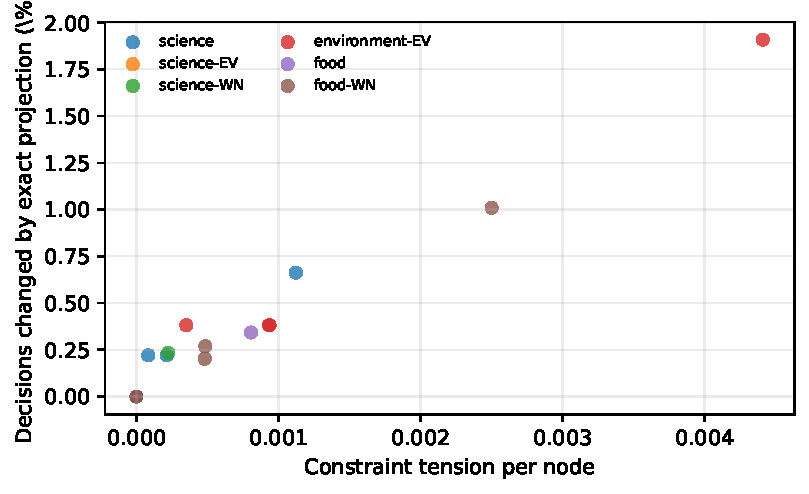
\includegraphics[width=0.82\columnwidth]{figures/constraint_tension.pdf}
\caption{Constraint tension predicts when exact decoding activates. Across
30 \method{} retraining--domain cells, tension per node and edit rate have Spearman
$\rho=\TensionChangeRho$. Scores are compared only within the same scorer.}
\label{fig:tension}
\end{figure}

\begin{table}[h]
\centering
\scriptsize
\setlength{\tabcolsep}{3pt}
\begin{tabular}{lccc}
\toprule
Decoder constraint & Macro4 \ef & Macro4 \af & Valid\\
\midrule
Exact forest & 38.07 & 40.87 & 100\\
No acyclicity & 38.05 & 40.25 & 60\\
No single-parent constraint & 36.87 & 39.71 & 0\\
\bottomrule
\end{tabular}
\caption{Frozen-potential decoder comparisons (percent). These rows change
the feasible family or its enforcement, not the neural evidence.}
\label{tab:ablations}
\end{table}

\begin{table}[h]
\centering
\scriptsize
\setlength{\tabcolsep}{3pt}
\begin{tabular}{lccc}
\toprule
Neural/policy variant & Macro4 \ef & Macro4 \af & Valid\\
\midrule
Confidence policy & 37.63 & 40.92 & 100\\
$-$ learned root & 20.75 & 19.82 & 100\\
$-$ typed potential penalties & 37.66 & 41.73 & 100\\
\bottomrule
\end{tabular}
\caption{Potential controls within the same development-tuned
root-budget family (percent); they are not compared as decoder ablations.}
\label{tab:potential-controls}
\end{table}

Replacing learned root evidence by uniform scores causes large, unstable
degradation within the root-budget family. The confidence-aware policy changes
9.30\% of decisions and lowers Macro6 \ef{} by 0.46 points. Removing its
hand-set typed penalties slightly raises \af{}, so typed classes are retained
as neural supervision and analysis rather than post-hoc symbolic weights.

\begin{table}[h]
\centering
\scriptsize
\setlength{\tabcolsep}{3pt}
\begin{tabular}{lrrrr}
\toprule
Domain & R@50 & \ef & \af & $\Delta$\af \\
\midrule
Science & 92.04 & 42.63$\pm$1.65 & 53.87$\pm$5.53 & +1.45 \\
Science-EV & 100.00 & 52.66$\pm$3.79 & 72.09$\pm$5.17 & 0.00 \\
Environment-EV & 80.08 & 35.94$\pm$3.71 & 23.22$\pm$1.48 & +1.00 \\
Food & 36.17 & 21.07$\pm$4.35 & 14.28$\pm$6.43 & $-$0.00 \\
\bottomrule
\end{tabular}
\caption{Primary system by external domain (confirmation retrainings, percent).
$\Delta$\af{} is exact branching minus independent learned-\rootnode{}
decoding; R@50 is candidate edge recall.}
\label{tab:domains}
\end{table}

\section{Additional Diagnostics}
\label{app:additional-diagnostics}

\begin{table}[h]
\centering
\small
\begin{tabular}{lrrr}
\toprule
Root decision & Precision & Recall & F1\\
\midrule
Standalone classifier & 5.22 & 55.85 & 8.59\\
Relation+\rootnode{} top-1 & 10.80 & 61.93 & 17.66\\
Relation+\rootnode{} exact & 10.93 & 64.43 & 17.91\\
\bottomrule
\end{tabular}
\caption{Macro4 root detection over 20 confirmatory retraining--domain cells
(percent). The standalone classifier overpredicts roots by 206.3 nodes per
graph on average; relation-root top-1 and exact overpredict by 132.4 and 132.8.
The standalone root probabilities have Brier score 0.054 and ECE 0.121.}
\label{tab:root-audit}
\end{table}

The root audit explains why learned root evidence supplies more hierarchy gain
than the final decode, yet remains the main calibration target. Exact
decoding slightly improves root F1 but cannot turn a poorly calibrated root
potential into semantic evidence.

\begin{table}[h]
\centering
\scriptsize
\setlength{\tabcolsep}{3pt}
\begin{tabular}{lrrr}
\toprule
Domain & Multi (\%) & One-parent & Cand.-limited\\
\midrule
Science & 2.88 & 98.47 & 94.44\\
Science-EV & 0.00 & 100.00 & 100.00\\
Environment-EV & 0.38 & 99.81 & 88.94\\
Food & 2.06 & 98.98 & 52.71\\
\midrule
Macro4 & -- & 99.32 & 84.02\\
\bottomrule
\end{tabular}
\caption{Exact \ef{} ceilings (percent). The candidate ceiling selects at most
one available gold parent per child; as a subgraph of the gold DAG, this
selection is acyclic and attainable by the output family.}
\label{tab:ceilings}
\end{table}

\begin{table}[h]
\centering
\small
\begin{tabular}{lrrr}
\toprule
Scoring execution & Test time & Pairs/s & Peak GPU\\
\midrule
Qwen3-8B & 848 s & 100.1 & 17.0 GB\\
Qwen3.5-27B & 4,789 s & 17.7 & 55.3 GB\\
\bottomrule
\end{tabular}
\caption{Batched forced-choice scoring of 84,860 test pairs with one model load.
Complete development-plus-test executions took 21.7 and 134.1 minutes.}
\label{tab:efficiency}
\end{table}

The DeBERTa-v3-base relation scorer has approximately 184M parameters, versus
27B for Qwen3.5-27B (about 147$\times$ fewer; retriever parameters excluded).
Replaying exact $k=20$ decoding from cached \method{} scores for all 30
retraining--domain graphs (22,535 nodes) takes 13.4 CPU seconds. Thus decoder
ablations reuse neural tensors and add negligible accelerator cost.

\section{Allocation Audits and Earlier Replications}
\label{app:allocation-audits}

\paragraph{Non-inferiority sensitivity.}
The edge lower bound is $+0.205$ points and passes even a zero-loss margin. The
ancestor lower bound is $-0.656$, so ancestor non-inferiority passes margins
0.75, 1.0, and 1.25 but not 0.5. Across four leave-one-domain-out analyses,
lower bounds range from $-0.073$ to $+0.415$ edge-F1 points and from $-0.901$
to $-0.432$ ancestor-F1 points, preserving the prespecified $-0.5/-1.0$
joint decision.

\paragraph{Earlier independent allocation evaluation.}
The the untouched retrainings with IDs 67--76 compare all allocation policies at exact
per-graph budgets. They are retained as an independent precursor to the
30-retraining non-inferiority replication.

\begin{table}[h]
\centering
\scriptsize
\setlength{\tabcolsep}{3pt}
\begin{tabular}{lrrr}
\toprule
Allocation policy & \ef & \af & Pairs\\
\midrule
Fixed $k=10$ & \PrimaryFixedEdge & \PrimaryFixedAncestor & 50\\
Random & \PrimaryRandomEdge & \PrimaryRandomAncestor & 75\\
Uniform budget & \PrimaryUniformEdge & \PrimaryUniformAncestor & 75\\
Symbolic only & \PrimarySymbolicEdge & \PrimarySymbolicAncestor & 75\\
Neural only & \PrimaryNeuralEdge & \PrimaryNeuralAncestor & 75\\
Combined & \PrimaryCombinedEdge & \PrimaryCombinedAncestor & 75\\
Full $k=20$ & \PrimaryFullEdge & \PrimaryFullAncestor & 100\\
\bottomrule
\end{tabular}
\caption{Earlier independent allocation evaluation, retraining IDs 67--76 (Macro4,
percent). Equal-budget policies score the same number of pairs in every graph;
all outputs are structurally valid.}
\label{tab:voc-initial}
\end{table}

\paragraph{Structured max-marginal allocation.}
Forced exclusion of a selected edge and forced inclusion of the strongest
unselected boundary edge define exact global decision gaps. A prespecified audit uses
these gaps as acquisition features without test labels or additional transformer
pair evaluations.

\begin{table}[h]
\centering
\scriptsize
\setlength{\tabcolsep}{3pt}
\begin{tabular}{lrrr}
\toprule
Allocation policy & \ef & \af & Pairs\\
\midrule
Fixed $k=10$ & \CertFixedEdge & \CertFixedAncestor & 50\\
Max-marginal only & \CertOnlyEdge & \CertOnlyAncestor & 75\\
Neural only & \CertNeuralEdge & \CertNeuralAncestor & 75\\
Local structural & \CertLocalEdge & \CertLocalAncestor & 75\\
Neural + max-marginal & \CertPlusEdge & \CertPlusAncestor & 75\\
Random & \CertRandomEdge & \CertRandomAncestor & 75\\
Uniform budget & \CertUniformEdge & \CertUniformAncestor & 75\\
Full $k=20$ & \CertFullEdge & \CertFullAncestor & 100\\
\bottomrule
\end{tabular}
\caption{Structured max-marginal allocation over independent retraining IDs 87--96
(Macro4 mean$\pm$SD, percent). The six middle rows have identical per-graph
pair budgets; every decoded output is structurally valid.}
\label{tab:certificate-allocation}
\end{table}

As secondary equal-budget contrasts, max-marginal-only improves random by
\CertOnlyMinusRandomEdge{} \ef{} points (95\% CI
[\CertOnlyMinusRandomEdgeLow, \CertOnlyMinusRandomEdgeHigh]) and uniform by
\CertOnlyMinusUniformAncestor{} \af{} points
([\CertOnlyMinusUniformAncestorLow, \CertOnlyMinusUniformAncestorHigh]); the
other endpoint in each comparison is inconclusive. The prespecified primary
contrast, neural-plus-max-marginal minus neural-only, is
\CertPlusMinusNeuralEdge{} \ef{}
([\CertPlusMinusNeuralEdgeLow, \CertPlusMinusNeuralEdgeHigh]) and
\CertPlusMinusNeuralAncestor{} \af{}
([\CertPlusMinusNeuralAncestorLow, \CertPlusMinusNeuralAncestorHigh]).
Against local structural allocation, the corresponding differences are
\CertPlusMinusLocalEdge{}
([\CertPlusMinusLocalEdgeLow, \CertPlusMinusLocalEdgeHigh]) and
\CertPlusMinusLocalAncestor{}
([\CertPlusMinusLocalAncestorLow, \CertPlusMinusLocalAncestorHigh]).
Thus the exact gaps are useful as a standalone audit-compatible signal, but
their additive value over learned gates is not established. All
\CertSeeds{} retraining manifests pass exact-budget, validity, and no-test-label
checks. Zero extra transformer pairs does not mean zero CPU work: computing
global gaps invokes repeated exact branching and is excluded from the headline
runtime-saving claim.

\paragraph{Protocol-separated allocation extensions.}
To distinguish structural information from correlation with neural
uncertainty, a graph-folded residual design first fits a neural gate on
development graphs; symbolic sensitivity features then predict only
$q_c-\widehat q_{c,\rm neural}^{\rm OOF}$. Its controls preserve neural scores and
per-graph budget while permuting the symbolic residual globally or within
neural-score deciles. A separate hierarchy-aware extension fits edge and
ancestor residual estimators and selects their weight on WordNet development
only. Finally, a large-pool audit exposes up to 200 dense candidates, assigns an
exact logical acquisition budget, deduplicates requested pairs, and scores them
in packed batches under one model load. We report logical acquisitions, unique
transformer-scored pairs, and measured runtime separately. These post-primary
analyses do not replace the untouched allocation result.

\begin{table}[h]
\centering
\scriptsize
\setlength{\tabcolsep}{3.2pt}
\begin{tabular}{lrrr}
\toprule
Scorer & Valid, before$\to$after & Edits & Correct/harm\\
\midrule
\method{} & 60.0$\to$100 & 42 (0.19\%) & 5 / 2\\
Qwen3-8B & 0.0$\to$100 & 304 (6.75\%) & 42 / 42\\
Qwen3.5-27B & 0.0$\to$100 & 152 (3.37\%) & 14 / 9\\
BoostTaxo-open & 16.7$\to$100 & 164 (3.64\%) & 12 / 17\\
\bottomrule
\end{tabular}
\caption{The same exact operator applied to four frozen scorers on all six
domains. Validity is the fraction of domain outputs; edit and correctness
counts are node decisions.}
\label{tab:cross-scorer}
\end{table}

\begin{table}[h]
\centering
\scriptsize
\setlength{\tabcolsep}{3pt}
\begin{tabular}{lrrr}
\toprule
Comparison & Exact & Neural$\to$exact & Conf.\\
\midrule
Changed decisions & 42 & 6,409 & 2,096\\
Changed rate & 0.19\% & 28.44\% & 9.30\%\\
Corrected / harmed & 5 / 2 & 500 / 833 & 92 / 93\\
Net corrections & +3 & $-$333 & $-$1\\
$\Delta$Macro6 \ef & +0.03 & $-$0.07 & $-$0.46\\
$\Delta$Macro4 \af & +0.62 & +4.11 & +0.67\\
Validity change & +40.0 & +100.0 & +40.0\\
\bottomrule
\end{tabular}
\caption{Confirmatory repair audit. ``Exact only'' compares learned-\rootnode{}
independent decoding with plain exact branching; ``end-to-end'' starts from
typed top-1 without \rootnode; ``confidence'' applies the tuned aggressive
policy after learned \rootnode. Deltas are percentage points.}
\label{tab:repair}
\end{table}

\paragraph{Hierarchy-allocation extension.}
A prespecified frozen-score analysis on retraining IDs 67--76 tests whether structural allocation
beats non-structural budget schedules under the same caches and external
domains. The symbolic allocator beats random by
\HierarchySymbolicMinusRandomEdge{} \ef{} points
(95\% CI [\HierarchySymbolicMinusRandomEdgeLow,
\HierarchySymbolicMinusRandomEdgeHigh]) and uniform by
\HierarchySymbolicMinusUniformEdge{} \ef{} points
([\HierarchySymbolicMinusUniformEdgeLow, \HierarchySymbolicMinusUniformEdgeHigh])
and \HierarchySymbolicMinusUniformAncestor{} \af{} points
([\HierarchySymbolicMinusUniformAncestorLow,
\HierarchySymbolicMinusUniformAncestorHigh]). The intervention audit shows a
\HierarchyNetRepairEnrichment{}-fold net repair enrichment
([\HierarchyNetRepairEnrichmentLow, \HierarchyNetRepairEnrichmentHigh]); the
symbolic allocator beats random on \HierarchySymbolicMinusRandomEdgeWins/10 retrainings
and the repair enrichment is positive on \HierarchyNetRepairEnrichmentWins/10
retrainings. All \HierarchyAuditValidOutputs{} decoded outputs are valid.

\paragraph{Earlier prespecified heuristic evaluation.}
Independent retrainings with IDs 52--56 used the thresholded union policy that
preceded the learned value-of-computation gate.

\begin{table}[h]
\centering
\scriptsize
\setlength{\tabcolsep}{3pt}
\begin{tabular}{lrrr}
\toprule
Allocation policy & \ef & \af & Pairs\\
\midrule
Fixed $k=10$ & \AdaptiveConfirmFixedEdge & \AdaptiveConfirmFixedAncestor & 50.00\\
Combined & \AdaptiveConfirmCombinedEdge & \AdaptiveConfirmCombinedAncestor & \AdaptiveConfirmPairFraction\\
Neural only & \AdaptiveConfirmNeuralEdge & \AdaptiveConfirmNeuralAncestor & \AdaptiveConfirmPairFraction\\
Symbolic only & \AdaptiveConfirmSymbolicEdge & \AdaptiveConfirmSymbolicAncestor & \AdaptiveConfirmPairFraction\\
Random & \AdaptiveConfirmRandomEdge & \AdaptiveConfirmRandomAncestor & \AdaptiveConfirmPairFraction\\
Uniform budget & \AdaptiveConfirmUniformEdge & \AdaptiveConfirmUniformAncestor & \AdaptiveConfirmPairFraction\\
Full $k=20$ reference & \AdaptiveConfirmFullEdge & \AdaptiveConfirmFullAncestor & 100.00\\
\bottomrule
\end{tabular}
\caption{All prespecified policies for independent retraining IDs 52--56 (Macro4
mean$\pm$SD, percent). The middle five rows have exactly equal scored-pair
counts in all \AdaptiveConfirmBudgetCells{} retraining--domain graphs. Bold marks the
best equal-budget mean, not a significant win over every control.}
\label{tab:adaptive-controls}
\end{table}

In this earlier evaluation, combined uses \AdaptiveConfirmCombinedPairs{} pairs
and \AdaptiveConfirmCombinedGPUSeconds{} mean CUDA seconds, versus
\AdaptiveConfirmFullPairs{} and \AdaptiveConfirmFullGPUSeconds{} for full
$k=20$. It improves \af{} over fixed $k=10$ by
\AdaptiveConfirmAncestorGain{} points
([\AdaptiveConfirmAncestorCILow, \AdaptiveConfirmAncestorCIHigh]) but does not
reduce wall time. We retain it as independent evidence rather than pooling its
five retrainings with the corrected learned-gate experiment.

\begin{table}[h]
\centering
\scriptsize
\setlength{\tabcolsep}{4pt}
\begin{tabular}{lrr}
\toprule
Domain & $\Delta$\ef & $\Delta$\af\\
\midrule
Science & \VoCScienceEdgeGain & \VoCScienceAncestorGain\\
Science-EuroVoc & \VoCScienceEVEdgeGain & \VoCScienceEVAncestorGain\\
Environment-EuroVoc & \VoCEnvironmentEVEdgeGain & \VoCEnvironmentEVAncestorGain\\
Food & \VoCFoodEdgeGain & \VoCFoodAncestorGain\\
Science-WordNet & \VoCScienceWNEdgeGain & \VoCScienceWNAncestorGain\\
Food-WordNet & \VoCFoodWNEdgeGain & \VoCFoodWNAncestorGain\\
\bottomrule
\end{tabular}
\caption{Corrected combined value-of-computation gate minus fixed $k=10$ by
domain (percentage points, retraining IDs 57--66). Macro4 excludes the two WordNet
self-tests; domain intervals are reported in the released aggregate.}
\label{tab:voc-domains}
\end{table}

\paragraph{Development precursor.}

\begin{table}[h]
\centering
\scriptsize
\setlength{\tabcolsep}{3pt}
\begin{tabular}{lrrr}
\toprule
Frozen-score decoder & \ef & \af & Pairs\\
\midrule
Exact, fixed $k=10$ & \AdaptiveFrozenBaseEdge & \AdaptiveFrozenBaseAncestor & 50.0\\
Gated $k=10\!\rightarrow\!20$ & \AdaptiveFrozenEdge & \AdaptiveFrozenAncestor & 77.95\\
\bottomrule
\end{tabular}
\caption{Post-freeze Macro4 analysis over retraining IDs 47--51 (mean$\pm$SD, percent).
The gate is selected only on node-disjoint WordNet development graphs. All
outputs are 100\% valid; pairs are the selected fraction of uniform $k=20$.}
\label{tab:adaptive}
\end{table}

The gate turns structural symptoms into a selective-computation policy while
the final exact decoder preserves the same hard guarantee. Because this
experiment replays a full frozen cache, pair fraction is a compute proxy rather
than a measured latency reduction, so it is not used for an efficiency claim.

\begin{table}[h]
\centering
\small
\begin{tabular}{lrr}
\toprule
Relation-scorer input & WordNet \ef & Valid\\
\midrule
Labels + glosses & \InputFull & 100.0\\
Labels only & \InputLabels & 100.0\\
Glosses only & \InputDefinitions & 100.0\\
Opaque node IDs + glosses & \InputAnonymous & 100.0\\
\bottomrule
\end{tabular}
\caption{Post-freeze input controls on 243 node-disjoint WordNet test graphs
over retraining IDs 47--51 (mean$\pm$SD, percent). Every mode uses the same frozen
$k=20$ candidate cache; one checkpoint load per retraining scores all four modes.}
\label{tab:input-controls}
\end{table}

The full input outperforms either channel alone, while masking lexical labels
causes the largest drop. These controls show complementary use of labels and
definitions and make a pure label-memorization explanation less plausible;
they cannot establish absence from pretraining corpora.

\section{Retraining Provenance}
\label{app:provenance}

\begin{table}[h]
\centering
\scriptsize
\setlength{\tabcolsep}{3pt}
\begin{tabular}{p{0.27\columnwidth}p{0.36\columnwidth}p{0.27\columnwidth}}
\toprule
Claim & Primary evidence & Does not claim\\
\midrule
Typed supervision & Retraining IDs 117--126; matched binary, pairwise, listwise & New
decoder guarantee\\
Exact constrained decoding & Retraining IDs 47--51; four scorers; pressure suite & Semantic
truth or candidate recovery\\
75\% pair budget & Retraining IDs 87--116; prespecified margins & Superiority to full
scoring\\
\bottomrule
\end{tabular}
\caption{Claim--evidence map. Each headline conclusion has a distinct control
and explicit boundary.}
\label{tab:evidence-map}
\end{table}

\begin{table}[h]
\centering
\scriptsize
\setlength{\tabcolsep}{1pt}
\begin{tabular}{p{0.16\columnwidth}p{0.30\columnwidth}p{0.43\columnwidth}}
\toprule
Retraining IDs & Role & Main-text claim\\
\midrule
42--46 & development & design and diagnostics only\\
47--51 & component confirmation & scorer/root/decoder decomposition\\
52--56 & fixed-protocol evaluation & thresholded allocation appendix\\
57--66 & corrected validation & implementation validation only\\
67--76 & initial confirmation & allocation precursor and controls\\
67--76 reuse & frozen-score extensions & hierarchy/pool analyses only\\
87--96 & matched objectives & semantic controls and transfer\\
87--96 & listwise robustness & additional matched semantic control\\
87--96 & max-marginal audit & global-gap allocation controls\\
87--116 & independent replication & compute non-inferiority\\
117--126 & equal-update matched objectives & matched semantic and transfer controls\\
\bottomrule
\end{tabular}
\caption{Non-pooled retraining roles. Retraining IDs 87--96 are a declared subset of the
30-retraining replication, not ten additional votes. The reuse row denotes a
separately specified analysis of frozen checkpoints or scores.}
\end{table}

Only retraining IDs 87--116 enter the headline non-inferiority test. Retraining IDs 87--96 also
support paired matched-control, transfer, listwise-robustness, and
max-marginal allocation analyses under separate manifests, but are counted once within each
contrast. Retraining IDs 67--76 provide independent precursor evidence and cannot vote
in the 30-retraining lower bounds. Development, corrected-validation, and reuse
analyses remain outside all headline confidence intervals. Retraining IDs 117--126
form a separate independent retraining replication and are not pooled with
retraining IDs 87--116. Their protocol was hash-locked before GPU outputs; this is not a
public preregistration. Before outcome inspection, an eligibility check was
corrected to admit the already specified retrainings with IDs 117--126. No computational field,
training code, checkpoint, candidate set, decoder, or metric changed. Executions for IDs
117--120 resumed from their existing checkpoints and root calibrations at the
TExEval stage and were not retrained.
The first large-pool launch was abandoned before metric inspection after a
cache audit found that $k\geq |V|$ could retain a masked self-candidate. The
corrected rerun adds an explicit finite non-self filter; neither
launch contributes to the independent replication.

\paragraph{Cache-only stress protocols.}
The release also includes two frozen-score stress analyses for the structural
claim. The constraint-pressure protocol boosts locally selected cyclic edges,
then records independent validity, exact validity, edit rate, constraint
tension, and task metrics. The expected mechanistic behavior is specific: as
pressure increases, independent decoding becomes less feasible, exact decoding
remains valid, edit rate and tension rise predictably, and changes stay
localized in the repair log.
The retrieval stress protocol decodes candidate prefixes at several depths and
reports candidate recall, a one-parent candidate ceiling, independent validity,
and exact validity. Both analyses reuse score tensors from retraining IDs 67--76, perform zero
transformer forwards, and use test labels only after decoding for metrics or
ceilings. Tables~\ref{tab:stress-projection}--\ref{tab:stress-regret-audit}
report mechanism-level decoder behavior rather than new state-of-the-art evidence.

\begin{table}[h]
\centering
\scriptsize
\setlength{\tabcolsep}{3pt}
\begin{tabular}{lrrrrrr}
\toprule
Pressure & Local valid & Exact valid & Edits & Tension/node & \ef & \af\\
\midrule
0.0 & \ProjectionStressBaseLocalValid & \ProjectionStressBaseExactValid &
\ProjectionStressBaseEditRate & \ProjectionStressBaseTension &
\ProjectionStressBaseEdge & \ProjectionStressBaseAncestor\\
2.0 & \ProjectionStressHighLocalValid & \ProjectionStressHighExactValid &
\ProjectionStressHighEditRate & \ProjectionStressHighTension &
\ProjectionStressHighEdge & \ProjectionStressHighAncestor\\
\bottomrule
\end{tabular}
\caption{Constraint-pressure audit on independent retraining IDs 67--76. Values are Macro4
means in percent except tension. The full grid is
$\{0,0.25,0.5,1,2\}$; all exact decodes are valid, and pressure--edit
association is $\rho=\ProjectionStressTensionEditSpearman$, matching the
constraint-tension account.}
\label{tab:stress-projection}
\end{table}

\begin{table}[h]
\centering
\scriptsize
\setlength{\tabcolsep}{3pt}
\begin{tabular}{rrrrrrr}
\toprule
$k$ & Cand. recall & Ceiling & Local valid & Exact valid & \ef & \af\\
\midrule
5 & \RetrievalStressKFiveRecall & \RetrievalStressKFiveCeiling &
\RetrievalStressKFiveLocalValid & \RetrievalStressKFiveExactValid &
\RetrievalStressKFiveEdge & \RetrievalStressKFiveAncestor\\
10 & \RetrievalStressKTenRecall & \RetrievalStressKTenCeiling &
\RetrievalStressKTenLocalValid & \RetrievalStressKTenExactValid &
\RetrievalStressKTenEdge & \RetrievalStressKTenAncestor\\
20 & \RetrievalStressKTwentyRecall & \RetrievalStressKTwentyCeiling &
\RetrievalStressKTwentyLocalValid & \RetrievalStressKTwentyExactValid &
\RetrievalStressKTwentyEdge & \RetrievalStressKTwentyAncestor\\
\bottomrule
\end{tabular}
\caption{Retrieval-prefix stress audit on independent retraining IDs 67--76 (Macro4 means,
percent). Exact decoding preserves feasibility at each candidate depth, while
semantic metrics track candidate availability and the one-parent candidate
ceiling.}
\label{tab:stress-retrieval}
\end{table}


\begin{table}[h]
\centering
\scriptsize
\setlength{\tabcolsep}{2pt}
\begin{tabular}{@{}lrrrrr@{}}
\toprule
Pressure & Cells & Bad local & Edits $\mu$/med & Tension $\mu$/med & Tension p90\\
\midrule
0.0 & \ProjectionAuditCells & \ProjectionAuditBaseInvalid &
\ProjectionAuditBaseEditsMean/\ProjectionAuditBaseEditsMedian &
\ProjectionAuditBaseTensionMean/\ProjectionAuditBaseTensionMedian &
\ProjectionAuditBaseTensionPninety\\
2.0 & \ProjectionAuditCells & \ProjectionAuditHighInvalid &
\ProjectionAuditHighEditsMean/\ProjectionAuditHighEditsMedian &
\ProjectionAuditHighTensionMean/\ProjectionAuditHighTensionMedian &
\ProjectionAuditHighTensionPninety\\
\bottomrule
\end{tabular}
\caption{Graph-level repair audit for the constraint-pressure protocol
(Macro4 cells, retraining IDs 67--76). Tension is
$T_\phi=S_\phi(\hat y)-S_\phi(y^*)$; edits are changed child decisions. Exact decoding restores
validity in all cells while tension grows under pressure and edits remain
localized.}
\label{tab:stress-regret-audit}
\end{table}

\section{Competing-Cycle Constraint Pressure}
\label{app:constraint-pressure-v2}

The second, independently sealed stress protocol generates disjoint and
overlapping competing cycles of lengths 2, 3, 5, and 8 at four node-pressure
levels on graphs of 64 and 128 nodes, with 20 deterministic replications per
cell. It uses no benchmark labels or transformer calls. ``Minimal edit'' first
minimizes the number of changes from independent decoding and only then
maximizes the frozen objective; exact decoding directly maximizes that objective.

\begin{table}[h]
\centering
\scriptsize
\setlength{\tabcolsep}{3pt}
\begin{tabular}{lrrrr}
\toprule
Decoder & Valid & Gap to optimum & Edits & Runtime (ms)\\
\midrule
Greedy repair & 100 & \PressureGreedyRegret & \PressureGreedyEdits & \PressureGreedyMillis\\
Minimal edit & 100 & \PressureMinimalRegret & \PressureMinimalEdits & \PressureMinimalMillis\\
Exact objective & \PressureExactValid & \PressureExactRegret & \PressureExactEdits & \PressureExactMillis\\
\bottomrule
\end{tabular}
\caption{Aggregate controlled constraint-pressure results over
\PressureRuns{} trials. The gap is $S_\phi(y^*)-S_\phi(y_m)$ for each feasible
decoder $m$; independent decoding is invalid in every deliberately pressured
instance. Exact decoding
uses slightly more edits when multiple cheap coordinated changes dominate one
expensive local repair, while preserving the original objective optimum.}
\label{tab:constraint-pressure-v2}
\end{table}

\section{Exact Selection Across Structural Families}
\label{app:family-selection}

The primary decoder fixes a feasible family and reports its constraint tension.
Multiple inheritance raises a different question: does the
available evidence justify changing the family itself?  We formalize that
question for nested families.  Let $\mathcal F_0$ contain single-parent
forests and let $\mathcal F_B\supseteq\mathcal F_0$ contain acyclic
taxonomies with at most two parents per child and at most $B$ second-parent
slots.  Write $A_s(y)$ for the unregularized additive evidence and
$M(y)$ for the number of used second-parent slots.  Define
\begin{align}
 P_B(s)&=\max_{y\in\mathcal F_B} A_s(y),\\
 R_B(s)&=P_B(s)-P_0(s),\label{eq:relaxation-value}\\
 L_B(s)&=\max_{y\in\mathcal L_B} A_s(y),\\
 T_B(s)&=L_B(s)-P_B(s).\label{eq:family-tension}
\end{align}
where $\mathcal L_B$ drops global acyclicity and budget coupling.
$R_B$ is the \emph{relaxation value}: neural score recovered by enlarging
the forest family. $T_B$ is the \emph{constraint tension}: score difference required
to enforce the declared global constraints.  They answer different questions.

Since $\mathcal F_0\subseteq\mathcal F_B\subseteq\mathcal L_B$,
$T_B,R_B\geq0$ and the identity
$L_B(s)-P_0(s)=T_B(s)+R_B(s)$ separates local evidence, global constraint
tension, and the score value of multiple inheritance.

Rather than report only two dev-selected thresholds, consider the complete
regularization path
\begin{align}
 y_\lambda&\in\argmax_{y\in\mathcal F_B}
 \{A_s(y)-\lambda M(y)\},\\
 V(\lambda)&=A_s(y_\lambda)-\lambda M(y_\lambda).
 \label{eq:family-path}
\end{align}
Positive $\lambda$ penalizes additional parents; negative $\lambda$ is an
explicit structural subsidy and is reported as such.

\begin{proposition}[Monotone structural path]
For $\lambda_1<\lambda_2$ and arbitrary optimizers at the two values,
$M(y_{\lambda_1})\geq M(y_{\lambda_2})$.  Moreover, $V(\lambda)$ is
convex and piecewise linear with an active slope $-M(y_\lambda)$.
\end{proposition}
\begin{proof}
Optimality at the two penalties gives
$A(y_1)-\lambda_1M(y_1)\geq A(y_2)-\lambda_1M(y_2)$ and
$A(y_2)-\lambda_2M(y_2)\geq A(y_1)-\lambda_2M(y_1)$.
Adding yields
$(\lambda_2-\lambda_1)(M(y_1)-M(y_2))\geq0$.
The value is the pointwise maximum of finitely many affine functions.
\end{proof}

The implementation obtains exact breakpoints from the cardinality frontier
$P_m=\max_{y:M(y)=m}A_s(y)$.  Cardinality $m$ is optimal precisely on
\begin{equation}
 \max_{j>m}\frac{P_j-P_m}{j-m}
 \;\leq\lambda\leq\;
 \min_{j<m}\frac{P_m-P_j}{m-j},
 \label{eq:penalty-interval}
\end{equation}
when this interval is nonempty.  These intervals certify that a reported
forest/DAG decision is not an artifact of a single threshold grid point.

\paragraph{Family-stability radius.}
Let $q(y)$ be the selected edge/ROOT indicator vector and let $y^*$ be the
current optimum.  Let $\gamma_{\rm fam}$ be its objective gap to the best
solution in the other family (forest versus any solution using a second
parent), and let
\begin{equation}
 D=\max_{y\text{ in other family}}\|q(y^*)-q(y)\|_1.
\end{equation}
Then
\begin{equation}
 \rho_{\rm fam}=\gamma_{\rm fam}/D
 \label{eq:family-radius}
\end{equation}
is a conservative family-stability radius: every perturbation
$\|\Delta s\|_\infty<\rho_{\rm fam}$ preserves the selected family.
Indeed, the score difference against every other-family solution decreases
by at most $\|\Delta s\|_\infty D<\gamma_{\rm fam}$.
Forced exclusion of a selected edge and forced inclusion of an unselected
second-parent decision similarly give edge-necessity and inclusion gaps.

\paragraph{A tractable ordered case.}
If every candidate edge respects a fixed strict topological order, any subset
is acyclic.  For each child, compute its best zero/one-parent value $b_c$ and
best two-parent value $d_c$, then select the at most $B$ largest positive
margins $d_c-b_c$.  This is globally exact because the budget is the only
remaining cross-child constraint.  It costs
$O(|E|+|V|\log|V|)$ for additive edge utilities, or
$O(\sum_c k_c^2+|V|\log|V|)$ with arbitrary parent-pair potentials.
The general cyclic candidate case retains the ILP decoder.

\paragraph{Evidence model and failure attribution.}
Raw single-parent ranking log-potentials are not variable-cardinality
probabilities.  Our revised pipeline therefore fits edge log-odds on WordNet
train, a child-level cardinality head, and a conditional parent-pair head.
The pair head ranks pairs after the first-parent evidence is known, while the
cardinality head decides whether the second slot is warranted.  WordNet dev
is reserved for ROOT calibration and $\lambda$ selection; the hard cap is a
predeclared structural limit rather than gold prevalence.

Retrieval remains an independent ceiling.  Among the
\MpOracleGoldChildren{} Macro4 multi-parent children, both gold parents occur
in the frozen top-20 pool for only
\MpOracleCompleteTwenty{} (\MpOracleCompleteTwentyRate\%) and in top-50 for
\MpOracleCompleteFifty{} (\MpOracleCompleteFiftyRate\%).  Food contributes
only \MpOracleFoodTwenty{} complete top-20 cases out of
\MpOracleFoodGold{}.  We consequently report four stages separately:
candidate-set coverage, cardinality detection, conditional second-parent
ranking, and exact globally feasible decoding.

\paragraph{Sealed semantic-pair follow-up.}
After inspecting the hybrid-retrieval and pair-oracle outcomes, we froze a
separate ten-seed follow-up; it cannot alter the primary branching or
allocation claims.  It reuses the coverage-preserving hybrid top-50 pools and
frozen 768-dimensional edge representations, requiring
\PairTransformerForwards{} additional transformer forwards.  For each child,
the scorer enumerates unordered pairs within the top-$q=20$ edge frontier and
uses the symmetric representation
\begin{equation}
 [h_i+h_j,\ |h_i-h_j|,\ h_i\odot h_j,\ \phi_{ij}],
\end{equation}
where $h_i$ is a learned transformation of frozen edge evidence and $\phi_{ij}$
contains symmetric scalar rank and score features.  The exact decoder sees
only the top-ranked pair ($M=1$), so the neural component must select the pair
and the symbolic component only enforces global DAG feasibility.

\begin{table}[h]
\centering
\scriptsize
\setlength{\tabcolsep}{3pt}
\begin{tabular}{lrrrrr}
\toprule
& \multicolumn{2}{c}{\ef} & \multicolumn{2}{c}{\af} & Pair R@1\\
\cmidrule(lr){2-3}\cmidrule(lr){4-5}
Scope & Hybrid & Sem.+margin & Hybrid & Sem.+margin & Scalar$\to$sem.\\
\midrule
Macro4 & \PairMacroFourBaselineEdge & \textbf{\PairMacroFourSemanticEdge} &
\PairMacroFourBaselineAncestor & \textbf{\PairMacroFourSemanticAncestor} &
\PairMacroFourScalarPairRecallOne$\rightarrow$\textbf{\PairMacroFourSemanticPairRecallOne}\\
Macro6 & \PairMacroSixBaselineEdge & \textbf{\PairMacroSixSemanticEdge} &
\PairMacroSixBaselineAncestor & \textbf{\PairMacroSixSemanticAncestor} &
\PairMacroSixScalarPairRecallOne$\rightarrow$\textbf{\PairMacroSixSemanticPairRecallOne}\\
\bottomrule
\end{tabular}
\caption{Post-outcome semantic parent-pair follow-up (mean percent, seeds
67--76). Pair R@1 is conditional on both gold parents occurring in the frozen
top-50 pool; its matched scalar control uses the same candidates and decoder.}
\label{tab:semantic-pair-followup}
\end{table}

On Macro4, semantic shortlisting improves \ef{} by
\PairMacroFourEdgeDelta{} points (95\% paired-seed bootstrap CI
[\PairMacroFourEdgeLow, \PairMacroFourEdgeHigh], exact sign-flip
$p=\PairMacroFourEdgeP$) and \af{} by \PairMacroFourAncestorDelta{} points
([\PairMacroFourAncestorLow, \PairMacroFourAncestorHigh],
$p=\PairMacroFourAncestorP$).  The edge effect is positive on
\PairMacroFourEdgeWins/\PairSeeds{} seeds.  Against the matched scalar pair
score, semantic pair recall@1 gains \PairMacroFourPairRecallDelta{} points
([\PairMacroFourPairRecallLow, \PairMacroFourPairRecallHigh],
$p=\PairMacroFourPairRecallP$).  Supporting Macro6 analysis shows
\PairMacroSixEdgeDelta/\PairMacroSixAncestorDelta{} \ef/\af{} gains
($p=\PairMacroSixEdgeP/\PairMacroSixAncestorP$) and a
\PairMacroSixPairRecallDelta-point pair-recall gain
($p=\PairMacroSixPairRecallP$).  Forest outputs are exactly unchanged, which
localizes these gains to semantic restriction of the multi-parent feasible
set.  Exact parent-set recovery is observed too rarely to support a positive
claim; the follow-up therefore establishes improved pair ranking and global
hierarchy reconstruction, not solved multiple inheritance.

\paragraph{Confirmatory joint-set budget ablation.}
We finally evaluate all predeclared pair frontiers with the joint
ROOT/singleton/pair scorer on a separate sealed set of
\JointSetSeeds{} seeds. A fixed frontier of $q=3$ scores only
\JointQThreePairs{} unordered pairs per child, compared with
\JointQFivePairs{} at $q=5$, \JointQTenPairs{} at $q=10$, and
\JointAdaptivePairs{} under uncertainty-adaptive allocation.

\begin{table}[h]
\centering
\scriptsize
\setlength{\tabcolsep}{3pt}
\begin{tabular}{llrrrr}
\toprule
Retrieval & Frontier & Pairs/child & Exact-set F1 & \ef & \af\\
\midrule
Hybrid40 & $q=3$ & \JointQThreePairs & \textbf{\JointHybridQThreeExact} &
\textbf{\JointHybridQThreeEdge} & \textbf{\JointHybridQThreeAncestor}\\
& $q=5$ & \JointQFivePairs & \JointHybridQFiveExact &
\JointHybridQFiveEdge & \JointHybridQFiveAncestor\\
& $q=10$ & \JointQTenPairs & \JointHybridQTenExact &
\JointHybridQTenEdge & \JointHybridQTenAncestor\\
& adaptive & \JointAdaptivePairs & \JointHybridAdaptiveExact &
\JointHybridAdaptiveEdge & \JointHybridAdaptiveAncestor\\
\midrule
Learned50 & $q=3$ & \JointQThreePairs & \textbf{\JointLearnedQThreeExact} &
\textbf{\JointLearnedQThreeEdge} & \textbf{\JointLearnedQThreeAncestor}\\
& $q=5$ & \JointQFivePairs & \JointLearnedQFiveExact &
\JointLearnedQFiveEdge & \JointLearnedQFiveAncestor\\
& $q=10$ & \JointQTenPairs & \JointLearnedQTenExact &
\JointLearnedQTenEdge & \JointLearnedQTenAncestor\\
& adaptive & \JointAdaptivePairs & \JointLearnedAdaptiveExact &
\JointLearnedAdaptiveEdge & \JointLearnedAdaptiveAncestor\\
\bottomrule
\end{tabular}
\caption{Confirmatory Macro4 joint-set budget ablation (mean percent, seeds
77--86). Bold marks the best mean within each retrieval pool; all rows retain
exact DAG feasibility.}
\label{tab:joint-set-budget}
\end{table}

The smallest frontier has the best mean exact-set, edge, and ancestor F1 in
both retrieval pools while reducing pair evaluation by
\JointQThreeSavingAdaptive\% relative to adaptive allocation,
\JointQThreeSavingQFive\% relative to $q=5$, and
\JointQThreeSavingQTen\% relative to $q=10$. We interpret this as a
descriptive efficiency result: wider pair enumeration provides no observed
benefit once the joint scorer has identified the strongest local frontier.
The preregistered exact-set contrast between Learned50+adaptive and
Hybrid40+$q=5$ is \JointPrimaryCandidateExact{} versus
\JointPrimaryReferenceExact{} F1 ($\Delta=\JointPrimaryExactDelta$ points,
Holm $p=\JointPrimaryExactP$), so it does not support a claim of improved
exact parent-set recovery.


\section{Post-Primary Multi-Parent DAG Extension}
\label{app:multiparent-dag}

The primary feasible family is deliberately single-parent because it admits a specialized maximum-branching optimizer. Exact DAG optimization with mixed-integer and topological-order formulations is established in Bayesian-network structure learning~\citep{park2017bayesian,decampos2011efficient}; our claim is therefore exact constrained selection across structural families, not ILP itself. We additionally test whether the
feasibility-and-repair interface survives a genuine change of feasible family. Let
$x_{cp}$ select candidate edge $c\to p$, let $z_c$ select \rootnode{}, and let
$m_c$ indicate use of a second parent. The post-primary ILP maximizes
\begin{equation}
 \sum_{c,p}s_{cp}x_{cp}+\sum_c r_cz_c-\tau_2\sum_c m_c
\end{equation}
subject to
\begin{align}
1-z_c &\leq \sum_p x_{cp}\leq 2(1-z_c),\\
\sum_p x_{cp}-1 &\leq m_c,\qquad \sum_p x_{cp}\geq2m_c,\\
\sum_c m_c &\leq B,
\end{align}
and MTZ topological-order constraints
$t_p\geq t_c+1-|V|(1-x_{cp})$. Thus every output is a DAG, every non-root has
one or two parents, and at most $B$ children use the second slot. The frozen potentials are ranking log-potentials trained for fixed-cardinality comparisons, not calibrated variable-cardinality probabilities. This original exploratory decoder therefore treats $\tau_2$ as a scale-correction threshold. Appendix~\ref{app:family-selection} replaces this heuristic with calibrated edge log-odds and explicit cardinality and pair evidence.

The same feasibility argument applies. Dropping acyclicity and the global
budget gives the independent per-child optimum $\hat y_2$ under the identical
objective. Exact ILP decoding reports the DAG constraint tension
\begin{equation}
T_{2,\phi}=S_\phi(\hat y_2)-\max_{y\in\mathcal F_{\rm DAG}}S_\phi(y).
\end{equation}
The implementation records a result only when HiGHS returns optimal status, an
independent verifier confirms all DAG constraints, and the itemized local
potential differences sum to $T_{2,\phi}$.

We reuse retraining IDs 67--76 score tensors with zero transformer forwards. The hard
cap is the WordNet-dev multi-parent prevalence
(\DagCapFraction\%); no external labels enter selection. We report two
dev-selected operating points from the same fixed threshold grid: one selected
lexicographically by overall \ef/\af{}, and one selected first by multi-parent
F1. This is explicitly post-primary and cannot alter the untouched allocation
claim.

\begin{table}[h]
\centering
\scriptsize
\setlength{\tabcolsep}{3pt}
\begin{tabular}{lrrrr}
\toprule
Decoder & \ef & \af & MP-child F1 & DAG valid\\
\midrule
Single-parent branching & \DagForestEdge & \DagForestAncestor & -- & 100\\
DAG, accuracy-selected & \DagAccuracyEdge & \DagAccuracyAncestor & 0.00 & 100\\
DAG, multi-parent-selected & \DagMultiEdge & \DagMultiAncestor & \DagMultiFone & 100\\
\bottomrule
\end{tabular}
\caption{Post-primary Macro4 means over retraining IDs 67--76 (percent). Both DAG rows
reuse the same frozen candidates and neural scores as the branching comparator.}
\label{tab:multiparent-dag}
\end{table}

All \DagValidOutputs{} primary-domain ILP outputs are proven optimal, acyclic,
and have independently verified feasibility records and itemized repair logs. Accuracy selection collapses to no
predicted second parents (nine of ten retrainings choose $\tau_2=0$), showing that
overall dev F1 does not support relaxing cardinality. The multi-parent-selected
operating point predicts \DagMultiPredicted{} multi-parent children per retraining
against \DagMultiGold{} gold, but only \DagMultiTruePositive{} correctly identify a gold multi-parent child on average: child-level cardinality precision/recall/F1 are
\DagMultiPrecision/\DagMultiRecall/\DagMultiFone\%. Its Macro4 change
relative to branching is \DagMultiEdgeDelta{} \ef{} points
(95\% CI [\DagMultiEdgeDeltaLow, \DagMultiEdgeDeltaHigh]) and
\DagMultiAncestorDelta{} \af{} points
([\DagMultiAncestorDeltaLow, \DagMultiAncestorDeltaHigh]). Hence the exact feasibility guarantee transfers to the broader DAG family, but this uncalibrated decoder-only objective does not recover parent sets.  It does not by itself distinguish retrieval failure, cardinality miscalibration, and conditional ranking error; Appendix~\ref{app:family-selection} provides that decomposition. A competitive
multi-parent system requires an explicit cardinality or conditional
second-parent model rather than a decoder-only relaxation.

\section{Reproducibility Checklist}

The released repository pins WordNet 3.0, TExEval-2 1.2, Schema.org 30.0,
Qwen3-Embedding-0.6B, and DeBERTa-v3-base. A locked dependency file and
Dockerfile specify the execution environment. Downloaded archives have expected
SHA-256 hashes and a receipt; the processed-data audit records removed synsets,
split assignments, class counts, and overlap assertions. Initialization IDs, optimizer
settings, early stopping, mixed precision, protocol seals, recovery commands,
and execution manifests are machine-readable.

Main tables are generated from JSON manifests without manual transcription.
The artifact exporter refuses to write numbers unless all 30 allocation
retrainings are present and both coprimary non-inferiority tests pass; it likewise
checks the ten matched-control, listwise, and transfer manifests and all ten max-marginal
manifests with signed receipts. Max-marginal protocol hashes, aggregate values,
equal budgets, validity, and no-test-label assertions are revalidated before
LaTeX macros are written. The restart audit preserves the unchanged evaluation
command. Decoder ablations share frozen score tensors, evidence partitions
remain separate, and
budget/resource checks are performed per graph. A content-addressed anonymous
artifact bundle includes source, protocols, Docker recipe, manifest, archive
SHA-256, and deposit metadata.

Anonymized source, protocols, manifests, and the Docker recipe are included
in the supplementary artifact. Its content manifest records per-file SHA-256
values; a public DOI will be minted only after the anonymity period.

\end{document}
